% Appendices A to D (Task 42). A: implementation (old A, t_impl with A8x / A6x lines); B: parameter randomisation
% (old A.1); C: near-duplicate analysis (old 5.6, t_limitations_*, t_neardup_split, t_sensitivity_*); D: supplementary
% results (old tables moved out of the main text, the A8 comparisons, the A8x / A6x records).
\appendix
\section{Implementation Details}
\label{sec:appendix}

Table~\ref{t_impl} lists the settings used on both datasets.
The FT-Transformer was trained with AdamW, a linear warm-up followed by cosine decay of the learning rate, gradient-norm
clipping, class weights proportional to the square root of the inverse class frequency (\apClassWeight), bf16
autocast during training and float32 for evaluation and attribution, and early stopping on validation macro-F1.
On 2018 all three seeds ran to the maximum of \apMaxEpochs{} epochs without early stopping (best epochs
\apBestEpochEighteen), and the validation macro-F1 ranged from \valFlatEighteenRange{} over the last
\apPatience{} epochs of every seed; on 2017 early stopping ended the runs after \apEpochsRunSeventeen{} epochs.
As a diagnostic of the attention explanations we selected, per seed, the single attention head (the [CLS] row of one
of the \apHeads{} heads in one of the \apBlocks{} layers) with the lowest deletion area under the curve (AUC) on the
validation explanation rows, macro-averaged over attack classes and with features masked by zero in the standardised
space, and evaluated it on the test explanation rows with training-mean masking like the other methods.
Features were log-transformed when non-negative with training skewness above the threshold, standardised with training
statistics and clipped.
Attacks used sign-gradient PGD with a cosine-decayed step size given as a fraction of the per-feature budget, the best
projected iterate per row over all steps and restarts, and one random restart.
The \nConsistency{} statistics of control c2 are the softmax entropy, energy, logit norm, the two largest logits and the
gap between the second and third, the benign logit, the largest attack-class logit, the logit standard deviation, the
benign probability, and the Mahalanobis and \paramKnn{}-nearest-neighbour distances for the predicted class.
Detector D used a very large inverse regularisation strength (effectively unregularised); D$_+$ used the value in the
table.
A8x computes IG in the loss with the same Gauss-Legendre rule as the true scores and was checked against the captum
implementation and against the saved true scores before any attack (Table~\ref{t_runs}); A6x runs over all test source
rows in chunks of the size used by A6, so that its random restart and batch shapes equal those of A6.

% Generated by paper_v3/gen/make_tables_v3.py on 2026-10-30. Do not edit.
% Source: paper_v3/generated/numbers.tex (macros ap*, param*, ax*, sx*)
\begin{table}[!tbp]
\centering
\footnotesize
\caption{Implementation settings (from the configuration, the attack scripts and the run logs).}
\label{t_impl}
\begin{tabular}{ll}
\toprule
Setting & Value \\
\midrule
\multicolumn{2}{l}{\textit{FT-Transformer}} \\
Width / blocks / heads & \apDModel{} / \apBlocks{} / \apHeads{} \\
Feed-forward factor & \apFfnFactor{} \\
Dropout (attention / feed-forward / residual) & \apAttnDropout{} / \apFfnDropout{} / \apResDropout{} \\
Learning rate / weight decay & \apLR{} / \apWeightDecay{} \\
Warm-up steps / batch size & \apWarmup{} / \apBatch{} \\
Maximum epochs / early-stopping patience & \apMaxEpochs{} / \apPatience{} \\
Gradient-norm clip & \apGradClip{} \\
Best epoch per seed, 2017 / 2018 & \apBestEpochSeventeen{} / \apBestEpochEighteen{} \\
Epochs run per seed, 2017 / 2018 & \apEpochsRunSeventeen{} / \apEpochsRunEighteen{} \\
Parameters (2018 model) & \apParamsEighteen{} \\
Log-transform skewness threshold / clip & \apSkewThr{} / \apClip{} \\
\midrule
\multicolumn{2}{l}{\textit{XGBoost}} \\
Maximum depth / learning rate & \apXgbDepth{} / \apXgbEta{} \\
Subsample / column subsample / minimum child weight & \apXgbSubsample{} / \apXgbColsample{} / \apXgbMinChild{} \\
Boosting rounds / early stopping & \apXgbRounds{} / \apXgbEarly{} \\
Best iteration, 2017 / 2018 & \apXgbBestSeventeen{} / \apXgbBestEighteen{} \\
\midrule
\multicolumn{2}{l}{\textit{Explanations}} \\
IG steps (explanations / detector scores) & \apIGSteps{} / \paramIGDet{} \\
IG benign baselines & \apIGBenignK{} \\
GradientSHAP background rows / samples & \apGsBackground{} / \apGsSamples{} \\
\midrule
\multicolumn{2}{l}{\textit{Constrained attacks}} \\
PGD steps / initial step size / restarts & \paramSteps{} / \apAlpha{} / \apRestarts{} \\
Budgets A0, A1, A1b, A2 & \apEpsList{} \\
Budgets A3 & \apEpsAthree{} \\
Unconstrained reference budgets (standardised) & \apEpsUnc{} \\
A2 margin floor / penalty & \apAtwoTau{} / \apAtwoPenalty{} \\
A3 margin cap & \apAthreeKappa{} \\
\midrule
\multicolumn{2}{l}{\textit{Defenders and adaptive attackers}} \\
kNN neighbours / reference rows per class & \paramKnn{} / \apKnnRef{} \\
Rows for the Mahalanobis covariance & \apMahaRows{} \\
D$_+$ inverse regularisation strength & \apCplus{} \\
A6 / A8 / A8x margin cap / hinge safety margin & \paramKappa{} / \apAsixSafety{} \\
Stand-in temperature / IG steps in the A8 loss & \apTau{} / \paramIGLoss{} \\
A8x: IG in the loss (Gauss-Legendre steps) & \axIGSteps{} \\
A8x: soft-rank temperature, annealed geometrically & \axTauStart{} to \axTauEnd{} \\
A8x / A6x: kept iterate, selection margin below the threshold & lowest true score / \axMargin{} \\
Rows per attack chunk, A6 / A8 (2018) / A8 (2017) & \apChunkAsix{} / \apChunkAeight{} / \apChunkAeightSeventeen{} \\
Rows per attack chunk, A8x / A6x & \axChunk{} / \sxChunk{} \\
\bottomrule
\end{tabular}
\end{table}


\section{Parameter Randomisation Check}
\label{sec:rand}
As a sanity check in the sense of \cite{adebayo2018}, we re-initialised parts of each trained FT-Transformer at
\nRandLevels{} levels (the classifier head alone; the transformer blocks cascading down from the last block, and then
also the feature tokenizer; and each block alone, with the classifier head kept) and recomputed the three attention
variants and IG on the first \randRowsPerClass{} rows per class of the clean explanation set.
Table~\ref{t_randomisation} gives, for three of these levels, the Spearman correlation and the top-\paramTopK{}
Jaccard overlap between the explanation of the original and of the randomised model.
With all blocks and the tokenizer re-initialised, the rollout ranking was unrelated to the original one (Spearman
\randRolloutAllSeventeen{} on 2017 and \randRolloutAllEighteen{} on 2018), and so was the signed IG
(\randIGSignedAllSeventeen{} and \randIGSignedAllEighteen), while the absolute IG kept a Spearman of
\randIGAbsAllSeventeen{} and \randIGAbsAllEighteen.
Re-initialising only the last block left rollout almost unchanged (\randRolloutTopOneSeventeen{} and
\randRolloutTopOneEighteen), which is expected because rollout also combines the attention of the unchanged lower
blocks, whereas the last-layer attention was no longer related to the original (\randLastTopOneSeventeen{} and
\randLastTopOneEighteen).
The attention explanations and the signed IG therefore changed when the learned weights were replaced; no
label-randomisation check was run.

% Generated by paper/make_tables_v2.py on 2026-10-30. Do not edit.
% Source: results/stage3_randomisation.csv
% Source: results/stage7/stage7c/stage7c_randomisation.csv
\begin{table}[t]
\centering
\footnotesize
\caption{Parameter randomisation check: similarity between the explanation of the original model and of the partly re-initialised model (7 common classes).}
\label{t_randomisation}
\sbox0{%
\begin{tabular}{lcccc}
\toprule
 & \multicolumn{2}{c}{2017} & \multicolumn{2}{c}{2018} \\
Explainer & Spearman & Jaccard@10 & Spearman & Jaccard@10 \\
\midrule
\multicolumn{5}{l}{\textit{Last block (block 3) re-initialised}} \\
Attn. rollout & $0.969$ {\scriptsize ($0.951$ to $0.978$)} & $0.890$ {\scriptsize ($0.872$ to $0.914$)} & $0.979$ {\scriptsize ($0.978$ to $0.981$)} & $0.901$ {\scriptsize ($0.891$ to $0.917$)} \\
Attn. layer mean & $0.938$ {\scriptsize ($0.918$ to $0.951$)} & $0.860$ {\scriptsize ($0.828$ to $0.883$)} & $0.947$ {\scriptsize ($0.942$ to $0.952$)} & $0.869$ {\scriptsize ($0.835$ to $0.909$)} \\
Attn. last layer & $0.041$ {\scriptsize ($-0.071$ to $0.145$)} & $0.100$ {\scriptsize ($0.076$ to $0.115$)} & $0.079$ {\scriptsize ($-0.147$ to $0.254$)} & $0.132$ {\scriptsize ($0.090$ to $0.190$)} \\
IG (absolute) & $0.711$ {\scriptsize ($0.633$ to $0.765$)} & $0.529$ {\scriptsize ($0.408$ to $0.618$)} & $0.770$ {\scriptsize ($0.758$ to $0.784$)} & $0.623$ {\scriptsize ($0.598$ to $0.644$)} \\
IG (signed) & $0.696$ {\scriptsize ($0.568$ to $0.800$)} & $0.533$ {\scriptsize ($0.409$ to $0.626$)} & $0.774$ {\scriptsize ($0.765$ to $0.790$)} & $0.626$ {\scriptsize ($0.612$ to $0.642$)} \\
\multicolumn{5}{l}{\textit{All blocks and the feature tokenizer re-initialised}} \\
Attn. rollout & $-0.067$ {\scriptsize ($-0.240$ to $0.043$)} & $0.084$ {\scriptsize ($0.072$ to $0.097$)} & $-0.051$ {\scriptsize ($-0.142$ to $0.066$)} & $0.045$ {\scriptsize ($0.018$ to $0.080$)} \\
IG (absolute) & $0.379$ {\scriptsize ($0.364$ to $0.392$)} & $0.195$ {\scriptsize ($0.162$ to $0.229$)} & $0.377$ {\scriptsize ($0.367$ to $0.384$)} & $0.183$ {\scriptsize ($0.160$ to $0.197$)} \\
IG (signed) & $0.028$ {\scriptsize ($-0.018$ to $0.079$)} & $0.157$ {\scriptsize ($0.154$ to $0.161$)} & $0.022$ {\scriptsize ($-0.015$ to $0.043$)} & $0.148$ {\scriptsize ($0.136$ to $0.156$)} \\
\multicolumn{5}{l}{\textit{First block (block 1) alone re-initialised}} \\
Attn. rollout & $0.044$ {\scriptsize ($-0.030$ to $0.174$)} & $0.108$ {\scriptsize ($0.085$ to $0.143$)} & $0.088$ {\scriptsize ($0.021$ to $0.206$)} & $0.084$ {\scriptsize ($0.060$ to $0.112$)} \\
IG (absolute) & $0.377$ {\scriptsize ($0.358$ to $0.411$)} & $0.181$ {\scriptsize ($0.176$ to $0.187$)} & $0.376$ {\scriptsize ($0.360$ to $0.390$)} & $0.187$ {\scriptsize ($0.141$ to $0.222$)} \\
\bottomrule
\end{tabular}}%
\ifdim\wd0>\textwidth\resizebox{\textwidth}{!}{\usebox0}\else\usebox0\fi
\par\smallskip\parbox{\linewidth}{\scriptsize Per row, on the first 50 rows per class of the clean explanation set (all rows of this subset), between the explanation of the trained model and that of a copy with the named parts re-initialised; the classifier head is kept. Spearman of the feature importances; Jaccard of the top-10 features. IG: training-mean baseline, original class; absolute IG is ranked by magnitude, signed IG by its signed value. Macro over the 7 common classes, mean over 3 seeds (seed range). Chance level of the top-10 Jaccard for 72 features: 0.078. Unchanged explanation: 1.}
\end{table}


\FloatBarrier
\section{Near-Duplicate Analysis}
\label{sec:sens}
Because the 2018 source rows had already been filtered for near duplicates, we decided before computing V1 that
cross-dataset comparisons should use rows without near duplicates; we fixed V1 as the primary set only after seeing the
sensitivity results.
Table~\ref{t_limitations_data} lists the small classes and the share of test rows with a
near duplicate in the training set, and Table~\ref{t_limitations_stages} the flagged source rows and benign test
negatives of the attack and detector experiments and the seeds of every pipeline step.
Table~\ref{t_neardup_split} compares rows with and without a near duplicate.
On 2017, flagged rows were easier for both detectors: on A6 rows ($\lambda = 1$) the TPR of D was \tprDNdSeventeen{} on
flagged and \tprDOtherSeventeen{} on other source rows (D$_+$: \tprDplusNdSeventeen{} and \tprDplusOtherSeventeen), and
the FPR of D was \fprDNdSeventeen{} on flagged and \fprDOtherSeventeen{} on other benign test negatives (D$_+$:
\fprDplusNdSeventeen{} and \fprDplusOtherSeventeen).
On 2018 no attack source row was flagged, and the FPR split was mixed: at $\epsilon = 1$, D \fprDNdEighteen{} on flagged
and \fprDOtherEighteen{} on other negatives (D$_+$: \fprDplusNdEighteen{} and \fprDplusOtherEighteen); at
$\epsilon = 0.5$, D \fprDNdEighteenHalf{} and \fprDOtherEighteenHalf{} (D$_+$: \fprDplusNdEighteenHalf{} and
\fprDplusOtherEighteenHalf).
Flagged rows made up \ndNegSeventeen{} and \ndNegEighteen{} of the benign test negatives.
Tables~\ref{t_sensitivity_2017_attacks} to~\ref{t_sensitivity_2018_defenders} give every attack and detector quantity on
V0, V1 and V2; their detector rows use D$_+$ against A8, the stand-in attacker.
Moving from V0 to V1 and V2 kept the levels of successful and undetected rows in their order of magnitude on both
datasets (2017 D under A6: \undetDAsixOneVzeroSeventeen, \undetDAsixOneVoneSeventeen, \undetDAsixOneVtwoSeventeen).

% Generated by paper/make_tables_v2.py on 2026-10-30. Do not edit.
% Source: results/stage3_randomisation.csv
% Source: results/stage7/stage7c/stage7c_3c_val_selection_counts.csv
% Source: results/stage7/stage7c/stage7c_randomisation.csv
% Source: results/stage7/stage7c/stage7c_selection_counts.csv
% Source: results/stage7/stage7d/stage7d_source_counts.csv
% Source: results/stage8/neardup_exact_2017_2018.csv
\begin{table}[t]
\centering
\footnotesize
\setlength{\tabcolsep}{4pt}
\caption{Limitations: small classes and near duplicates of test rows.}
\label{t_limitations_data}
\resizebox{\textwidth}{!}{%
\begin{tabular}{llll}
\toprule
Dataset / set & Detail & Class / n & Value \\
\midrule
\multicolumn{4}{l}{\textit{Classes with fewer than 100 rows per seed}} \\
2018 & clean explanation set (test) & Web attack & $85$ \\
2018 & VAL explanation set (head choice, defender positives) & Web attack & $84$ \\
2018 & attack and defender source rows & Web attack & $85$ \\
2017 & randomisation subset (by design) & every class & $50$ \\
2018 & randomisation subset (by design) & every class & $50$ \\
2018 & randomisation subset & DoS Slowloris without near duplicates & $37$ \\
\midrule
\multicolumn{4}{l}{{\begin{tabular}[t]{@{}l@{}}\textit{Test rows within $10^{-3}$ of a train row (standardised space,}\\\textit{exact distance to the nearest train row; share of test rows)}\end{tabular}}} \\
2017 & DoS Slowloris & 1{,}027 & $0.351$ \\
2017 & Bot & 144 & $0.000$ \\
2017 & DDoS & 18{,}754 & $0.000$ \\
2017 & DoS GoldenEye & 1{,}326 & $0.000$ \\
2017 & DoS Hulk & 31{,}158 & $0.001$ \\
2017 & SSH-Patator & 580 & $0.000$ \\
2017 & Web attack & 397 & $0.411$ \\
2017 & all test rows (any class) & 302{,}327 & $0.108$ \\
2018 & DoS Slowloris & 1{,}809 & $0.456$ \\
2018 & Bot & 19{,}220 & $0.002$ \\
2018 & DDoS & 60{,}000 & $0.000$ \\
2018 & DoS GoldenEye & 5{,}373 & $0.000$ \\
2018 & DoS Hulk & 60{,}000 & $0.000$ \\
2018 & SSH-Patator & 18{,}524 & $0.000$ \\
2018 & Web attack & 85 & $0.000$ \\
2018 & all test rows (any class) & 365{,}011 & $0.043$ \\
\bottomrule
\end{tabular}}
\par\smallskip\parbox{\linewidth}{\scriptsize The randomisation check uses 50 rows per class by design. Near duplicates: every test row of both datasets against every train row of the same dataset, direct squared differences (no matrix-product expansion), distance to the nearest row computed in float64.}
\end{table}

% Generated by paper/make_tables_v2.py on 2026-10-30. Do not edit.
% Source: results/stage2_per_class_f1.csv
% Source: results/stage3_faithfulness.csv
% Source: results/stage3_randomisation.csv
% Source: results/stage3c_faithfulness.csv
% Source: results/stage5
% Source: results/stage6/final
% Source: results/stage6/strong
% Source: results/stage7
% Source: results/stage7/stage7c/stage7c_3c_faithfulness.csv
% Source: results/stage7/stage7c/stage7c_faithfulness.csv
% Source: results/stage7/stage7c/stage7c_randomisation.csv
% Source: results/stage7/stage7d
% Source: results/stage7/stage7e
% Source: results/stage9/ablation/2017/stageA_defenders.csv
% Source: results/stage9/ablation/2018/stageA_defenders.csv
% Source: results/stage8/sensitivity_flags.csv
% Source: results/stage8/sensitivity_negatives.csv
\begin{table}[t]
\centering
\footnotesize
\caption{Limitations: near-duplicate source rows and negatives of the attack and defender experiments, and seeds per pipeline step.}
\label{t_limitations_stages}
\begin{tabular}{llll}
\toprule
Dataset / set & Detail & Class / n & Value \\
\midrule
\multicolumn{4}{l}{{\begin{tabular}[t]{@{}l@{}}\textit{Near-duplicate source rows of the attack and defender experiments}\\\textit{(per seed; the same rows in every attack and defender experiment)}\end{tabular}}} \\
2017 & DoS Hulk & 1 of 150 & $0.007$ \\
2017 & DoS Slowhttptest & 128 of 150 & $0.853$ \\
2017 & DoS Slowloris & 73 of 150 & $0.487$ \\
2017 & Web attack & 69 of 150 & $0.460$ \\
2017 & all attack classes & 271 of 1{,}494 & $0.181$ \\
2018 & all attack classes & 0 of 985 & $0.000$ \\
\midrule
\multicolumn{4}{l}{{\begin{tabular}[t]{@{}l@{}}\textit{Benign test negatives of the defenders (1{,}000 per seed): near-duplicate share}\\\textit{and FPR at $\epsilon = 1$ on near-duplicate vs other negatives (D / D$_+$)}\end{tabular}}} \\
2017 & negatives, pooled over seeds & 385 of 3{,}000 & $0.128$ \\
2017 & FPR on near-duplicate negatives &  & $0.008$ / $0.016$ \\
2017 & FPR on the other negatives &  & $0.059$ / $0.058$ \\
2018 & negatives, pooled over seeds & 217 of 3{,}000 & $0.072$ \\
2018 & FPR on near-duplicate negatives &  & $0.060$ / $0.037$ \\
2018 & FPR on the other negatives &  & $0.054$ / $0.050$ \\
\midrule
\multicolumn{4}{l}{\textit{Seeds used in each pipeline step}} \\
2017 & FT-T training & 0, 1, 2 &  \\
2017 & Clean explanations & 0, 1, 2 &  \\
2017 & Explanation diagnostics & 0, 1, 2 &  \\
2017 & Parameter randomisation & 0, 1, 2 &  \\
2017 & Constrained attacks & 0, 1, 2 &  \\
2017 & Defenders D and D$_+$ & 0, 1, 2 &  \\
2017 & Adaptive attack A8 & 0, 1, 2 &  \\
2017 & Controls for D$_+$ & 0, 1, 2 &  \\
2018 & FT-T training & 0, 1, 2 &  \\
2018 & Clean explanations & 0, 1, 2 &  \\
2018 & Explanation diagnostics & 0, 1, 2 &  \\
2018 & Parameter randomisation & 0, 1, 2 &  \\
2018 & Constrained attacks & 0, 1, 2 &  \\
2018 & Defenders D and D$_+$; attacks A6, A8 & 0, 1, 2 &  \\
2018 & Controls for D$_+$ & 0, 1, 2 &  \\
\bottomrule
\end{tabular}
\end{table}

% Generated by paper/make_tables_v2.py on 2026-10-30. Do not edit.
% Source: results/stage8/sensitivity_negatives.csv
% Source: results/stage8/neardup_rows_{2017,2018}.parquet
% Source: results/stage6/final/seed{0,1,2}/rows_eps*_*.parquet and results/stage6/strong/seed{0,1,2}/rows_eps1_A8*.parquet (7 common classes)
% Source: results/stage7/stage7e/seed{0,1,2}/rows_eps*_*.parquet
\begin{table}[t]
\centering
\footnotesize
\caption{Detection of rows with and without a near duplicate in train.}
\label{t_neardup_split}
\begin{tabular}{llllllll}
\toprule
 &  &  & \multicolumn{2}{c}{D} & \multicolumn{2}{c}{D$_+$} &  \\
Dataset & $\epsilon$ & Quantity & Flagged & Other & Flagged & Other & n flagged / other \\
\midrule
2017 & $1.0$ & TPR, A6 $\lambda{=}1$ rows & $0.918$ & $0.589$ & $0.957$ & $0.827$ & 328 / 1{,}341 \\
2017 & $1.0$ & TPR, A8 $\lambda{=}1$ rows & $0.983$ & $0.692$ & $0.904$ & $0.732$ & 356 / 1{,}417 \\
2017 & $1.0$ & FPR, benign test negatives & $0.008$ & $0.059$ & $0.016$ & $0.058$ & 385 / 2{,}615 \\
2017 & $0.5$ & TPR, A6 $\lambda{=}1$ rows & $1.000$ & $0.995$ & $1.000$ & $0.995$ & 147 / 392 \\
2017 & $0.5$ & TPR, A8 $\lambda{=}1$ rows & n/a & n/a & n/a & n/a & 0 / 0 \\
2017 & $0.5$ & FPR, benign test negatives & $0.016$ & $0.059$ & $0.023$ & $0.061$ & 385 / 2{,}615 \\
\midrule
2018 & $1.0$ & TPR, A6 $\lambda{=}1$ rows & n/a & $0.955$ & n/a & $0.992$ & 0 / 896 \\
2018 & $1.0$ & TPR, A8 $\lambda{=}1$ rows & n/a & $0.980$ & n/a & $0.963$ & 0 / 991 \\
2018 & $1.0$ & FPR, benign test negatives & $0.060$ & $0.054$ & $0.037$ & $0.050$ & 217 / 2{,}783 \\
2018 & $0.5$ & TPR, A6 $\lambda{=}1$ rows & n/a & $1.000$ & n/a & $0.998$ & 0 / 450 \\
2018 & $0.5$ & TPR, A8 $\lambda{=}1$ rows & n/a & $0.998$ & n/a & $0.991$ & 0 / 429 \\
2018 & $0.5$ & FPR, benign test negatives & $0.212$ & $0.045$ & $0.055$ & $0.044$ & 217 / 2{,}783 \\
\bottomrule
\end{tabular}
\par\smallskip\parbox{\linewidth}{\scriptsize Flagged: the test row has a train row within $10^{-3}$ (exact distance, standardised space). TPR is computed on source rows that the attack flipped to benign (7 common classes, all source rows, pooled over seeds); FPR on the benign test negatives of the defenders, pooled over seeds. n/a: no flagged row, or no A8 run at that budget. Thresholds at 5\% FPR on validation benign rows.}
\end{table}

% Generated by paper/make_tables_v2.py on 2026-10-30. Do not edit.
% Source: results/stage8/sensitivity_stage5.csv
% Source: results/stage8/sensitivity_defenders.csv
% Source: results/stage8/sensitivity_paired.csv
% Source: results/stage8/sensitivity_union.csv
% Source: results/stage8/sensitivity_checks.csv
\begin{table}[t]
\centering
\footnotesize
\setlength{\tabcolsep}{5pt}
\caption{Near-duplicate sensitivity, constrained attacks, 2017 (7 common classes): all source rows (V0), near duplicates removed (V1), slowloris and web attack removed (V2).}
\label{t_sensitivity_2017_attacks}
\sbox0{%
\begin{tabular}{lccc}
\toprule
Quantity & V0 & V1 & V2 \\
\midrule
\multicolumn{4}{l}{\textit{Constrained attacks (mean over seeds)}} \\
Source rows per seed & 1044 & 901 & 744 \\
A1 success, $\epsilon = 1$ & {\begin{tabular}[t]{@{}c@{}}$0.649$\\{\scriptsize ($0.490$ to $0.811$)}\end{tabular}} & {\begin{tabular}[t]{@{}c@{}}$0.622$\\{\scriptsize ($0.461$ to $0.814$)}\end{tabular}} & {\begin{tabular}[t]{@{}c@{}}$0.617$\\{\scriptsize ($0.458$ to $0.766$)}\end{tabular}} \\
A0 success, $\epsilon = 1$ & {\begin{tabular}[t]{@{}c@{}}$0.198$\\{\scriptsize ($0.104$ to $0.276$)}\end{tabular}} & {\begin{tabular}[t]{@{}c@{}}$0.206$\\{\scriptsize ($0.103$ to $0.270$)}\end{tabular}} & {\begin{tabular}[t]{@{}c@{}}$0.137$\\{\scriptsize ($0.043$ to $0.209$)}\end{tabular}} \\
A1 minus A0, $\epsilon = 0.5$ & {\begin{tabular}[t]{@{}c@{}}$0.126$\\{\scriptsize ($0.052$ to $0.221$)}\end{tabular}} & {\begin{tabular}[t]{@{}c@{}}$0.089$\\{\scriptsize ($0.002$ to $0.228$)}\end{tabular}} & {\begin{tabular}[t]{@{}c@{}}$0.094$\\{\scriptsize ($0.005$ to $0.147$)}\end{tabular}} \\
A1 minus A0, $\epsilon = 1.0$ & {\begin{tabular}[t]{@{}c@{}}$0.451$\\{\scriptsize ($0.276$ to $0.543$)}\end{tabular}} & {\begin{tabular}[t]{@{}c@{}}$0.416$\\{\scriptsize ($0.216$ to $0.544$)}\end{tabular}} & {\begin{tabular}[t]{@{}c@{}}$0.480$\\{\scriptsize ($0.298$ to $0.584$)}\end{tabular}} \\
A2 mass ratio, $\epsilon = 0.5$ & {\begin{tabular}[t]{@{}c@{}}$0.943$\\{\scriptsize ($0.915$ to $0.963$)}\end{tabular}} & {\begin{tabular}[t]{@{}c@{}}$0.946$\\{\scriptsize ($0.911$ to $0.967$)}\end{tabular}} & {\begin{tabular}[t]{@{}c@{}}$0.957$\\{\scriptsize ($0.931$ to $0.975$)}\end{tabular}} \\
A2 mass ratio, $\epsilon = 1.0$ & {\begin{tabular}[t]{@{}c@{}}$0.902$\\{\scriptsize ($0.870$ to $0.943$)}\end{tabular}} & {\begin{tabular}[t]{@{}c@{}}$0.906$\\{\scriptsize ($0.864$ to $0.948$)}\end{tabular}} & {\begin{tabular}[t]{@{}c@{}}$0.927$\\{\scriptsize ($0.901$ to $0.953$)}\end{tabular}} \\
A3 $\lambda{=}1000$ mass ratio, $\epsilon = 0.5$ & {\begin{tabular}[t]{@{}c@{}}$0.938$\\{\scriptsize ($0.904$ to $0.963$)}\end{tabular}} & {\begin{tabular}[t]{@{}c@{}}$0.941$\\{\scriptsize ($0.898$ to $0.966$)}\end{tabular}} & {\begin{tabular}[t]{@{}c@{}}$0.950$\\{\scriptsize ($0.915$ to $0.975$)}\end{tabular}} \\
A3 $\lambda{=}1000$ mass ratio, $\epsilon = 1.0$ & {\begin{tabular}[t]{@{}c@{}}$0.896$\\{\scriptsize ($0.861$ to $0.940$)}\end{tabular}} & {\begin{tabular}[t]{@{}c@{}}$0.900$\\{\scriptsize ($0.855$ to $0.947$)}\end{tabular}} & {\begin{tabular}[t]{@{}c@{}}$0.915$\\{\scriptsize ($0.880$ to $0.945$)}\end{tabular}} \\
Flipped A1, margin AOPC gap minus A0, IG & {\begin{tabular}[t]{@{}c@{}}$-10.70$\\{\scriptsize ($-12.78$ to $-8.83$)}\end{tabular}} & {\begin{tabular}[t]{@{}c@{}}$-11.06$\\{\scriptsize ($-13.04$ to $-9.02$)}\end{tabular}} & {\begin{tabular}[t]{@{}c@{}}$-10.73$\\{\scriptsize ($-12.73$ to $-8.92$)}\end{tabular}} \\
Flipped A1, margin AOPC gap minus A0, rollout & {\begin{tabular}[t]{@{}c@{}}$-7.61$\\{\scriptsize ($-8.90$ to $-6.23$)}\end{tabular}} & {\begin{tabular}[t]{@{}c@{}}$-7.45$\\{\scriptsize ($-8.09$ to $-6.59$)}\end{tabular}} & {\begin{tabular}[t]{@{}c@{}}$-6.73$\\{\scriptsize ($-7.73$ to $-5.81$)}\end{tabular}} \\
Flipped A1, margin AOPC gap minus A0, static rollout & {\begin{tabular}[t]{@{}c@{}}$-5.49$\\{\scriptsize ($-5.98$ to $-4.56$)}\end{tabular}} & {\begin{tabular}[t]{@{}c@{}}$-5.43$\\{\scriptsize ($-6.16$ to $-4.63$)}\end{tabular}} & {\begin{tabular}[t]{@{}c@{}}$-4.63$\\{\scriptsize ($-5.10$ to $-4.34$)}\end{tabular}} \\
\bottomrule
\end{tabular}}%
\ifdim\wd0>\textwidth\resizebox{\textwidth}{!}{\usebox0}\else\usebox0\fi
\par\smallskip\parbox{\linewidth}{\scriptsize V0: all source rows (reproduces the attack and defender tables). V1: source rows whose test row has a train row within $10^{-3}$ removed in both datasets. V2: DoS Slowloris and Web attack removed in both datasets (5 classes). Rows are filtered after the fact: attacks, models and defenders (trained on validation) are unchanged. Mean (seed range); defender rows and differences: pooled over rows with the paired bootstrap 95\% CI, union also with the per-seed range.}
\end{table}

% Generated by paper/make_tables_v2.py on 2026-10-30. Do not edit.
% Source: results/stage8/sensitivity_stage5.csv
% Source: results/stage8/sensitivity_defenders.csv
% Source: results/stage8/sensitivity_paired.csv
% Source: results/stage8/sensitivity_union.csv
% Source: results/stage8/sensitivity_checks.csv
\begin{table}[t]
\centering
\footnotesize
\setlength{\tabcolsep}{5pt}
\caption{Near-duplicate sensitivity, defenders, 2017 (7 common classes): all source rows (V0), near duplicates removed (V1), slowloris and web attack removed (V2).}
\label{t_sensitivity_2017_defenders}
\sbox0{%
\begin{tabular}{lccc}
\toprule
Quantity & V0 & V1 & V2 \\
\midrule
\multicolumn{4}{l}{\textit{Defenders at $\epsilon = 1$ (pooled over rows, seed range)}} \\
A1 success (share of source rows) & {\begin{tabular}[t]{@{}c@{}}$0.648$\\{\scriptsize ($0.489$ to $0.810$)}\end{tabular}} & {\begin{tabular}[t]{@{}c@{}}$0.620$\\{\scriptsize ($0.459$ to $0.795$)}\end{tabular}} & {\begin{tabular}[t]{@{}c@{}}$0.615$\\{\scriptsize ($0.456$ to $0.765$)}\end{tabular}} \\
Undet.\ D, A6 $\lambda{=}1$ & {\begin{tabular}[t]{@{}c@{}}$0.185$\\{\scriptsize ($0.127$ to $0.250$)}\end{tabular}} & {\begin{tabular}[t]{@{}c@{}}$0.204$\\{\scriptsize ($0.148$ to $0.272$)}\end{tabular}} & {\begin{tabular}[t]{@{}c@{}}$0.226$\\{\scriptsize ($0.179$ to $0.294$)}\end{tabular}} \\
Undet.\ D$_+$, A8 $\lambda{=}1$ & {\begin{tabular}[t]{@{}c@{}}$0.132$\\{\scriptsize ($0.060$ to $0.267$)}\end{tabular}} & {\begin{tabular}[t]{@{}c@{}}$0.141$\\{\scriptsize ($0.064$ to $0.277$)}\end{tabular}} & {\begin{tabular}[t]{@{}c@{}}$0.155$\\{\scriptsize ($0.078$ to $0.290$)}\end{tabular}} \\
Undet.\ D$_+$, A8 $\lambda{=}100$ & {\begin{tabular}[t]{@{}c@{}}$0.127$\\{\scriptsize ($0.011$ to $0.298$)}\end{tabular}} & {\begin{tabular}[t]{@{}c@{}}$0.125$\\{\scriptsize ($0.012$ to $0.279$)}\end{tabular}} & {\begin{tabular}[t]{@{}c@{}}$0.122$\\{\scriptsize ($0.015$ to $0.253$)}\end{tabular}} \\
TPR D$_+$ minus D, A6 $\lambda{=}1$ rows & {\begin{tabular}[t]{@{}c@{}}$0.199$\\{\scriptsize [$0.177$, $0.219$]}\end{tabular}} & {\begin{tabular}[t]{@{}c@{}}$0.238$\\{\scriptsize [$0.213$, $0.265$]}\end{tabular}} & {\begin{tabular}[t]{@{}c@{}}$0.271$\\{\scriptsize [$0.241$, $0.299$]}\end{tabular}} \\
TPR D$_+$ minus D, A8 $\lambda{=}1$ rows & {\begin{tabular}[t]{@{}c@{}}$0.016$\\{\scriptsize [$-0.005$, $0.039$]}\end{tabular}} & {\begin{tabular}[t]{@{}c@{}}$0.040$\\{\scriptsize [$0.013$, $0.066$]}\end{tabular}} & {\begin{tabular}[t]{@{}c@{}}$0.072$\\{\scriptsize [$0.042$, $0.101$]}\end{tabular}} \\
TPR D$_+$ minus D, A8 $\lambda{=}100$ rows & {\begin{tabular}[t]{@{}c@{}}$-0.047$\\{\scriptsize [$-0.074$, $-0.022$]}\end{tabular}} & {\begin{tabular}[t]{@{}c@{}}$-0.017$\\{\scriptsize [$-0.049$, $0.013$]}\end{tabular}} & {\begin{tabular}[t]{@{}c@{}}$0.028$\\{\scriptsize [$-0.008$, $0.065$]}\end{tabular}} \\
TPR D$_+$ minus D, A8 norm. rows & {\begin{tabular}[t]{@{}c@{}}$-0.012$\\{\scriptsize [$-0.032$, $0.007$]}\end{tabular}} & {\begin{tabular}[t]{@{}c@{}}$0.013$\\{\scriptsize [$-0.010$, $0.034$]}\end{tabular}} & {\begin{tabular}[t]{@{}c@{}}$0.049$\\{\scriptsize [$0.023$, $0.077$]}\end{tabular}} \\
Equal-effort union, D$_+$ minus D & {\begin{tabular}[t]{@{}c@{}}$-0.025$\\{\scriptsize [$-0.039$, $-0.012$]}\\{\scriptsize ($-0.089$ to $0.063$)}\end{tabular}} & {\begin{tabular}[t]{@{}c@{}}$-0.037$\\{\scriptsize [$-0.050$, $-0.023$]}\\{\scriptsize ($-0.084$ to $0.031$)}\end{tabular}} & {\begin{tabular}[t]{@{}c@{}}$-0.049$\\{\scriptsize [$-0.065$, $-0.033$]}\\{\scriptsize ($-0.071$ to $-0.004$)}\end{tabular}} \\
\bottomrule
\end{tabular}}%
\ifdim\wd0>\textwidth\resizebox{\textwidth}{!}{\usebox0}\else\usebox0\fi
\par\smallskip\parbox{\linewidth}{\scriptsize Rows, row sets and intervals as in Table~\ref{t_sensitivity_2017_attacks}.}
\end{table}

% Generated by paper/make_tables_v2.py on 2026-10-30. Do not edit.
% Source: results/stage8/sensitivity_stage5.csv
% Source: results/stage8/sensitivity_defenders.csv
% Source: results/stage8/sensitivity_paired.csv
% Source: results/stage8/sensitivity_union.csv
% Source: results/stage8/sensitivity_checks.csv
\begin{table}[t]
\centering
\footnotesize
\setlength{\tabcolsep}{5pt}
\caption{Near-duplicate sensitivity, constrained attacks, 2018: all source rows (V0), near duplicates removed (V1), slowloris and web attack removed (V2).}
\label{t_sensitivity_2018_attacks}
\sbox0{%
\begin{tabular}{lccc}
\toprule
Quantity & V0 & V1 & V2 \\
\midrule
\multicolumn{4}{l}{\textit{Constrained attacks (mean over seeds)}} \\
Source rows per seed & 985 & 985 & 750 \\
A1 success, $\epsilon = 1$ & {\begin{tabular}[t]{@{}c@{}}$0.601$\\{\scriptsize ($0.294$ to $0.866$)}\end{tabular}} & {\begin{tabular}[t]{@{}c@{}}$0.601$\\{\scriptsize ($0.294$ to $0.866$)}\end{tabular}} & {\begin{tabular}[t]{@{}c@{}}$0.618$\\{\scriptsize ($0.267$ to $0.904$)}\end{tabular}} \\
A0 success, $\epsilon = 1$ & {\begin{tabular}[t]{@{}c@{}}$0.185$\\{\scriptsize ($0.087$ to $0.317$)}\end{tabular}} & {\begin{tabular}[t]{@{}c@{}}$0.185$\\{\scriptsize ($0.087$ to $0.317$)}\end{tabular}} & {\begin{tabular}[t]{@{}c@{}}$0.147$\\{\scriptsize ($0.031$ to $0.285$)}\end{tabular}} \\
A1 minus A0, $\epsilon = 0.5$ & {\begin{tabular}[t]{@{}c@{}}$0.082$\\{\scriptsize ($-0.004$ to $0.160$)}\end{tabular}} & {\begin{tabular}[t]{@{}c@{}}$0.082$\\{\scriptsize ($-0.004$ to $0.160$)}\end{tabular}} & {\begin{tabular}[t]{@{}c@{}}$0.136$\\{\scriptsize ($0.028$ to $0.243$)}\end{tabular}} \\
A1 minus A0, $\epsilon = 1.0$ & {\begin{tabular}[t]{@{}c@{}}$0.416$\\{\scriptsize ($0.207$ to $0.550$)}\end{tabular}} & {\begin{tabular}[t]{@{}c@{}}$0.416$\\{\scriptsize ($0.207$ to $0.550$)}\end{tabular}} & {\begin{tabular}[t]{@{}c@{}}$0.471$\\{\scriptsize ($0.236$ to $0.619$)}\end{tabular}} \\
A2 mass ratio, $\epsilon = 0.5$ & {\begin{tabular}[t]{@{}c@{}}$0.917$\\{\scriptsize ($0.907$ to $0.927$)}\end{tabular}} & {\begin{tabular}[t]{@{}c@{}}$0.917$\\{\scriptsize ($0.907$ to $0.927$)}\end{tabular}} & {\begin{tabular}[t]{@{}c@{}}$0.921$\\{\scriptsize ($0.911$ to $0.934$)}\end{tabular}} \\
A2 mass ratio, $\epsilon = 1.0$ & {\begin{tabular}[t]{@{}c@{}}$0.861$\\{\scriptsize ($0.840$ to $0.874$)}\end{tabular}} & {\begin{tabular}[t]{@{}c@{}}$0.861$\\{\scriptsize ($0.840$ to $0.874$)}\end{tabular}} & {\begin{tabular}[t]{@{}c@{}}$0.866$\\{\scriptsize ($0.839$ to $0.885$)}\end{tabular}} \\
A3 $\lambda{=}1000$ mass ratio, $\epsilon = 0.5$ & {\begin{tabular}[t]{@{}c@{}}$0.926$\\{\scriptsize ($0.917$ to $0.941$)}\end{tabular}} & {\begin{tabular}[t]{@{}c@{}}$0.926$\\{\scriptsize ($0.917$ to $0.941$)}\end{tabular}} & {\begin{tabular}[t]{@{}c@{}}$0.923$\\{\scriptsize ($0.912$ to $0.934$)}\end{tabular}} \\
A3 $\lambda{=}1000$ mass ratio, $\epsilon = 1.0$ & {\begin{tabular}[t]{@{}c@{}}$0.869$\\{\scriptsize ($0.854$ to $0.885$)}\end{tabular}} & {\begin{tabular}[t]{@{}c@{}}$0.869$\\{\scriptsize ($0.854$ to $0.885$)}\end{tabular}} & {\begin{tabular}[t]{@{}c@{}}$0.871$\\{\scriptsize ($0.860$ to $0.885$)}\end{tabular}} \\
Flipped A1, margin AOPC gap minus A0, IG & {\begin{tabular}[t]{@{}c@{}}$-11.36$\\{\scriptsize ($-12.05$ to $-10.99$)}\end{tabular}} & {\begin{tabular}[t]{@{}c@{}}$-11.36$\\{\scriptsize ($-12.05$ to $-10.99$)}\end{tabular}} & {\begin{tabular}[t]{@{}c@{}}$-11.09$\\{\scriptsize ($-11.32$ to $-10.82$)}\end{tabular}} \\
Flipped A1, margin AOPC gap minus A0, rollout & {\begin{tabular}[t]{@{}c@{}}$-7.50$\\{\scriptsize ($-8.93$ to $-5.84$)}\end{tabular}} & {\begin{tabular}[t]{@{}c@{}}$-7.50$\\{\scriptsize ($-8.93$ to $-5.84$)}\end{tabular}} & {\begin{tabular}[t]{@{}c@{}}$-6.74$\\{\scriptsize ($-7.89$ to $-4.58$)}\end{tabular}} \\
Flipped A1, margin AOPC gap minus A0, static rollout & {\begin{tabular}[t]{@{}c@{}}$-6.19$\\{\scriptsize ($-7.39$ to $-4.99$)}\end{tabular}} & {\begin{tabular}[t]{@{}c@{}}$-6.19$\\{\scriptsize ($-7.39$ to $-4.99$)}\end{tabular}} & {\begin{tabular}[t]{@{}c@{}}$-6.65$\\{\scriptsize ($-7.29$ to $-5.44$)}\end{tabular}} \\
\bottomrule
\end{tabular}}%
\ifdim\wd0>\textwidth\resizebox{\textwidth}{!}{\usebox0}\else\usebox0\fi
\par\smallskip\parbox{\linewidth}{\scriptsize Rows, row sets and intervals as in Table~\ref{t_sensitivity_2017_attacks}.}
\end{table}

% Generated by paper/make_tables_v2.py on 2026-10-30. Do not edit.
% Source: results/stage8/sensitivity_stage5.csv
% Source: results/stage8/sensitivity_defenders.csv
% Source: results/stage8/sensitivity_paired.csv
% Source: results/stage8/sensitivity_union.csv
% Source: results/stage8/sensitivity_checks.csv
\begin{table}[t]
\centering
\footnotesize
\setlength{\tabcolsep}{5pt}
\caption{Near-duplicate sensitivity, defenders, 2018: all source rows (V0), near duplicates removed (V1), slowloris and web attack removed (V2).}
\label{t_sensitivity_2018_defenders}
\sbox0{%
\begin{tabular}{lccc}
\toprule
Quantity & V0 & V1 & V2 \\
\midrule
\multicolumn{4}{l}{\textit{Defenders at $\epsilon = 1$ (pooled over rows, seed range)}} \\
A1 success (share of source rows) & {\begin{tabular}[t]{@{}c@{}}$0.584$\\{\scriptsize ($0.266$ to $0.863$)}\end{tabular}} & {\begin{tabular}[t]{@{}c@{}}$0.584$\\{\scriptsize ($0.266$ to $0.863$)}\end{tabular}} & {\begin{tabular}[t]{@{}c@{}}$0.618$\\{\scriptsize ($0.267$ to $0.904$)}\end{tabular}} \\
Undet.\ D, A6 $\lambda{=}1$ & {\begin{tabular}[t]{@{}c@{}}$0.014$\\{\scriptsize ($0.002$ to $0.036$)}\end{tabular}} & {\begin{tabular}[t]{@{}c@{}}$0.014$\\{\scriptsize ($0.002$ to $0.036$)}\end{tabular}} & {\begin{tabular}[t]{@{}c@{}}$0.017$\\{\scriptsize ($0.001$ to $0.047$)}\end{tabular}} \\
Undet.\ D$_+$, A8 $\lambda{=}1$ & {\begin{tabular}[t]{@{}c@{}}$0.013$\\{\scriptsize ($0.001$ to $0.020$)}\end{tabular}} & {\begin{tabular}[t]{@{}c@{}}$0.013$\\{\scriptsize ($0.001$ to $0.020$)}\end{tabular}} & {\begin{tabular}[t]{@{}c@{}}$0.016$\\{\scriptsize ($0.000$ to $0.027$)}\end{tabular}} \\
Undet.\ D$_+$, A8 $\lambda{=}100$ & {\begin{tabular}[t]{@{}c@{}}$0.013$\\{\scriptsize ($0.001$ to $0.018$)}\end{tabular}} & {\begin{tabular}[t]{@{}c@{}}$0.013$\\{\scriptsize ($0.001$ to $0.018$)}\end{tabular}} & {\begin{tabular}[t]{@{}c@{}}$0.016$\\{\scriptsize ($0.000$ to $0.024$)}\end{tabular}} \\
TPR D$_+$ minus D, A6 $\lambda{=}1$ rows & {\begin{tabular}[t]{@{}c@{}}$0.037$\\{\scriptsize [$0.021$, $0.051$]}\end{tabular}} & {\begin{tabular}[t]{@{}c@{}}$0.037$\\{\scriptsize [$0.021$, $0.051$]}\end{tabular}} & {\begin{tabular}[t]{@{}c@{}}$0.048$\\{\scriptsize [$0.029$, $0.066$]}\end{tabular}} \\
TPR D$_+$ minus D, A8 $\lambda{=}1$ rows & {\begin{tabular}[t]{@{}c@{}}$-0.017$\\{\scriptsize [$-0.032$, $-0.003$]}\end{tabular}} & {\begin{tabular}[t]{@{}c@{}}$-0.017$\\{\scriptsize [$-0.032$, $-0.003$]}\end{tabular}} & {\begin{tabular}[t]{@{}c@{}}$-0.026$\\{\scriptsize [$-0.047$, $-0.006$]}\end{tabular}} \\
TPR D$_+$ minus D, A8 $\lambda{=}100$ rows & {\begin{tabular}[t]{@{}c@{}}$-0.016$\\{\scriptsize [$-0.031$, $0.001$]}\end{tabular}} & {\begin{tabular}[t]{@{}c@{}}$-0.016$\\{\scriptsize [$-0.031$, $0.001$]}\end{tabular}} & {\begin{tabular}[t]{@{}c@{}}$-0.022$\\{\scriptsize [$-0.042$, $-0.001$]}\end{tabular}} \\
TPR D$_+$ minus D, A8 norm. rows & {\begin{tabular}[t]{@{}c@{}}$-0.012$\\{\scriptsize [$-0.018$, $-0.006$]}\end{tabular}} & {\begin{tabular}[t]{@{}c@{}}$-0.012$\\{\scriptsize [$-0.018$, $-0.006$]}\end{tabular}} & {\begin{tabular}[t]{@{}c@{}}$-0.015$\\{\scriptsize [$-0.024$, $-0.008$]}\end{tabular}} \\
Equal-effort union, D$_+$ minus D & {\begin{tabular}[t]{@{}c@{}}$-0.001$\\{\scriptsize [$-0.008$, $0.007$]}\\{\scriptsize ($-0.050$ to $0.029$)}\end{tabular}} & {\begin{tabular}[t]{@{}c@{}}$-0.001$\\{\scriptsize [$-0.008$, $0.007$]}\\{\scriptsize ($-0.050$ to $0.029$)}\end{tabular}} & {\begin{tabular}[t]{@{}c@{}}$0.000$\\{\scriptsize [$-0.010$, $0.010$]}\\{\scriptsize ($-0.067$ to $0.040$)}\end{tabular}} \\
\bottomrule
\end{tabular}}%
\ifdim\wd0>\textwidth\resizebox{\textwidth}{!}{\usebox0}\else\usebox0\fi
\par\smallskip\parbox{\linewidth}{\scriptsize Rows, row sets and intervals as in Table~\ref{t_sensitivity_2017_attacks}.}
\end{table}


\FloatBarrier
\section{Supplementary Results}
\label{sec:supp}

\paragraph{Attacks by budget and all source rows.}
Figure~\ref{f_evasion_eps} and Table~\ref{t_evasion} give constrained evasion success by budget, and
Tables~\ref{t_clean_agreement}, \ref{t_clean_faith} and~\ref{t_faith_attack} the clean-data and attack tables of the
main text on all rows (V0) next to V1, with the A3 variants and budgets that the main text omits.
Table~\ref{t_defenders} and Table~\ref{t_per_class} give the detector results per attack and per class on all source
rows (V0), and Figures~\ref{f_detection_tpr} and~\ref{f_per_class_heatmap} the corresponding TPR and per-class union;
in these, D$_+$ faces the stand-in attacker A8.

\paragraph{Clean-data results that did not replicate.}
Three results on 2017 did not hold in the same direction on 2018 (all explanation-set rows): the advantage of a static
class-mean rollout ranking over the per-row ranking (AOPC gap of static minus per-row rollout \staticGapSeventeen{},
seed range \staticGapSeventeenRange, against \staticGapEighteen, \staticGapEighteenRange); the advantage of $|x|$ over
rollout (deletion rank \rankDelAbsXSeventeen{} and \rankDelAbsXEighteen{} for $|x|$, \rankDelRolloutSeventeen{} and
\rankDelRolloutEighteen{} for rollout); and the advantage of the single attention head selected on validation data
(difference to rollout \headMinusRolloutSeventeen, seed range \headMinusRolloutSeventeenRange, against
\headMinusRolloutEighteen, \headMinusRolloutEighteenRange).
The method orderings on V0 and V2 correlated across the datasets with \ordSpDelVzero{} and \ordSpDelVtwo{} (deletion)
and \ordSpInsVzero{} and \ordSpInsVtwo{} (insertion).

\paragraph{Against the stand-in attacker A8.}
Table~\ref{t_union_a8} gives the equal-effort union with D$_+$ facing A8 on all row sets, and the comparison of each
control with D$_+$ under A8.
The 2017 difference D$_+$ minus D under A8 was \axStandinVzeroSeventeen{} (\axStandinVzeroSeventeenCI) on V0,
\axStandinVoneSeventeen{} (\axStandinVoneSeventeenCI) on V1 and \axStandinVtwoSeventeen{} (\axStandinVtwoSeventeenCI) on
V2, and the paired TPR difference on A8 rows changed sign with the row set for some settings (for $\lambda = 100$:
\tprAeightHundredVzeroSeventeen, \tprAeightHundredVoneSeventeen, \tprAeightHundredVtwoSeventeen).
The control columns of Table~\ref{t_union_a8} compare each control with D$_+$ under the stand-in attacker; they are
not a comparison at the stronger attacker, which is in Table~\ref{t_union_adaptive}.
The stand-ins reproduced the true consistency scores with a median $R^2$ of \standinMedSeventeenRange{} on 2017 and
\standinMedEighteenRange{} on 2018 across seeds; Table~\ref{t_standin} gives every score for A8 and for the attackers
of a1 and a2.

\paragraph{A8x and A6x.}
Table~\ref{t_a8x_setting} gives D$_+$ minus D under A8x per attack setting, the unequal-effort sensitivity unions and
the A6x union, and Table~\ref{t_a8x_tpr} the paired TPR and AUROC differences on the A8x and A8 rows on every row set.
With the A8 and A8x candidates together against D$_+$, an unequal-effort sensitivity union that favours the attacker of
D$_+$, the 2017 difference was \axSensVoneSeventeen{} (\axSensVoneSeventeenCI); with A6 and A6x together against D it
was \sxSensVoneSeventeen{} (\sxSensVoneSeventeenCI).
Table~\ref{t_runs} records the runs: rows, invalid rows, time, memory and the sanity checks that compared the
quantities computed inside A8x and A6x with the saved values before any attack.
The first sanity run of A8x failed at tolerance $10^{-5}$ on the Mahalanobis score and the D$_+$ decision, from
single-precision noise of the batch shape; the tolerance was set to $10^{-3}$ for these two quantities and the
\axMargin{} selection margin added before any pilot or attack, and the margin changed the in-loop count of
undetected rows from \axInloopNoMarginSeventeen{} to \axInloopMarginSeventeen{} on 2017 and no evaluated row.
The first sanity run of A6x, at a chunk smaller than that of A6, changed the path of \sxRunoneRows{} of the checked rows;
at the chunk of A6 it reproduced the saved A6 rows exactly, and A6x was run at that chunk.

\begin{figure*}[!tbp]
  \centering
  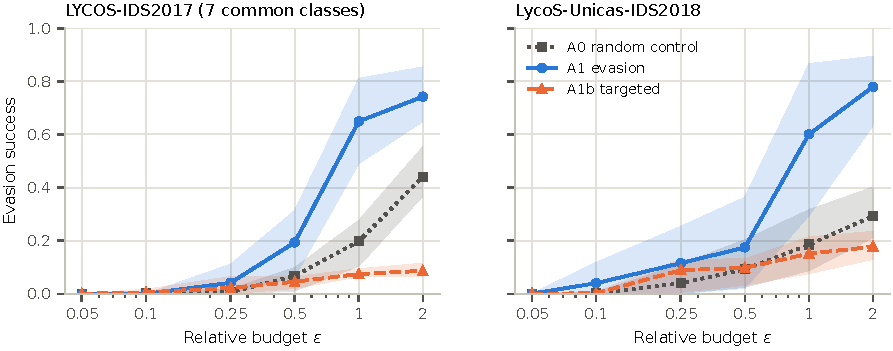
\includegraphics[width=\textwidth]{f_evasion_eps}
  \caption{Constrained evasion success by budget (bands: seed range).}
  \label{f_evasion_eps}
\end{figure*}

% Generated by paper/make_tables_v2.py on 2026-10-30. Do not edit.
% Source: results/stage7/stage7d/cmp2017_seed0_success.csv
% Source: results/stage7/stage7d/cmp2017_seed1_success.csv
% Source: results/stage7/stage7d/cmp2017_seed2_success.csv
% Source: results/stage7/stage7d/seed0/summary_success.csv
% Source: results/stage7/stage7d/seed1/summary_success.csv
% Source: results/stage7/stage7d/seed2/summary_success.csv
\begin{table}[t]
\centering
\footnotesize
\caption{Constrained evasion success by budget, 2017 vs 2018 (7 common classes).}
\label{t_evasion}
\begin{tabular}{lcc}
\toprule
Budget & 2017 mean (seed range) & 2018 mean (seed range) \\
\midrule
\multicolumn{3}{l}{\textit{A0}} \\
$\epsilon = 0.05$ & $0.000$ {\scriptsize ($0.000$ to $0.001$)} & $0.000$ {\scriptsize ($0.000$ to $0.000$)} \\
$\epsilon = 0.10$ & $0.003$ {\scriptsize ($0.000$ to $0.010$)} & $0.002$ {\scriptsize ($0.000$ to $0.005$)} \\
$\epsilon = 0.25$ & $0.006$ {\scriptsize ($0.000$ to $0.018$)} & $0.040$ {\scriptsize ($0.002$ to $0.111$)} \\
$\epsilon = 0.50$ & $0.067$ {\scriptsize ($0.010$ to $0.099$)} & $0.092$ {\scriptsize ($0.025$ to $0.204$)} \\
$\epsilon = 1.00$ & $0.198$ {\scriptsize ($0.104$ to $0.276$)} & $0.185$ {\scriptsize ($0.087$ to $0.317$)} \\
$\epsilon = 2.00$ & $0.439$ {\scriptsize ($0.368$ to $0.554$)} & $0.293$ {\scriptsize ($0.211$ to $0.402$)} \\
\multicolumn{3}{l}{\textit{A1}} \\
$\epsilon = 0.05$ & $0.000$ {\scriptsize ($0.000$ to $0.000$)} & $0.001$ {\scriptsize ($0.001$ to $0.001$)} \\
$\epsilon = 0.10$ & $0.000$ {\scriptsize ($0.000$ to $0.000$)} & $0.040$ {\scriptsize ($0.001$ to $0.118$)} \\
$\epsilon = 0.25$ & $0.042$ {\scriptsize ($0.001$ to $0.111$)} & $0.115$ {\scriptsize ($0.001$ to $0.254$)} \\
$\epsilon = 0.50$ & $0.193$ {\scriptsize ($0.063$ to $0.313$)} & $0.175$ {\scriptsize ($0.021$ to $0.364$)} \\
$\epsilon = 1.00$ & $0.649$ {\scriptsize ($0.490$ to $0.811$)} & $0.601$ {\scriptsize ($0.294$ to $0.866$)} \\
$\epsilon = 2.00$ & $0.742$ {\scriptsize ($0.649$ to $0.854$)} & $0.779$ {\scriptsize ($0.633$ to $0.895$)} \\
\multicolumn{3}{l}{\textit{A1b}} \\
$\epsilon = 0.05$ & $0.000$ {\scriptsize ($0.000$ to $0.001$)} & $0.000$ {\scriptsize ($0.000$ to $0.000$)} \\
$\epsilon = 0.10$ & $0.006$ {\scriptsize ($0.000$ to $0.017$)} & $0.003$ {\scriptsize ($0.000$ to $0.008$)} \\
$\epsilon = 0.25$ & $0.022$ {\scriptsize ($0.000$ to $0.065$)} & $0.089$ {\scriptsize ($0.006$ to $0.130$)} \\
$\epsilon = 0.50$ & $0.045$ {\scriptsize ($0.020$ to $0.065$)} & $0.098$ {\scriptsize ($0.032$ to $0.131$)} \\
$\epsilon = 1.00$ & $0.075$ {\scriptsize ($0.065$ to $0.094$)} & $0.151$ {\scriptsize ($0.076$ to $0.214$)} \\
$\epsilon = 2.00$ & $0.087$ {\scriptsize ($0.065$ to $0.115$)} & $0.177$ {\scriptsize ($0.130$ to $0.235$)} \\
\bottomrule
\end{tabular}
\par\smallskip\parbox{\linewidth}{\scriptsize Success: A0 any change of prediction, A1 predicted benign, A1b predicted as the target class. Macro over the 7 common classes, mean over 3 seeds. $\epsilon = 2$ is the stress setting. A1b targets differ for 3 classes on 2018 (the 2017 targets are absent).}
\end{table}

% Generated by paper/make_tables_v2.py on 2026-10-30. Do not edit.
% Source: results/stage7/stage7c/stage7c_cmp2017_agreement.csv
% Source: results/stage8/clean_variants.csv
\begin{table}[t]
\centering
\footnotesize
\caption{Clean-data agreement, 2017 vs 2018 (7 common classes): Spearman between attention and attribution rankings, all explanation rows (V0) and without near duplicates (V1).}
\label{t_clean_agreement}
\sbox0{%
\begin{tabular}{lcccc}
\toprule
 & \multicolumn{2}{c}{2017} & \multicolumn{2}{c}{2018} \\
Quantity & V0 & V1 & V0 & V1 \\
\midrule
Attn. rollout vs IG & {\begin{tabular}[t]{@{}c@{}}$0.357$\\{\scriptsize ($0.339$ to $0.378$)}\end{tabular}} & {\begin{tabular}[t]{@{}c@{}}$0.349$\\{\scriptsize ($0.317$ to $0.373$)}\end{tabular}} & {\begin{tabular}[t]{@{}c@{}}$0.323$\\{\scriptsize ($0.244$ to $0.423$)}\end{tabular}} & {\begin{tabular}[t]{@{}c@{}}$0.314$\\{\scriptsize ($0.244$ to $0.406$)}\end{tabular}} \\
Attn. rollout vs GradientSHAP & {\begin{tabular}[t]{@{}c@{}}$0.475$\\{\scriptsize ($0.422$ to $0.507$)}\end{tabular}} & {\begin{tabular}[t]{@{}c@{}}$0.470$\\{\scriptsize ($0.412$ to $0.505$)}\end{tabular}} & {\begin{tabular}[t]{@{}c@{}}$0.438$\\{\scriptsize ($0.366$ to $0.523$)}\end{tabular}} & {\begin{tabular}[t]{@{}c@{}}$0.432$\\{\scriptsize ($0.365$ to $0.515$)}\end{tabular}} \\
Attn. rollout vs Occlusion & {\begin{tabular}[t]{@{}c@{}}$0.399$\\{\scriptsize ($0.364$ to $0.433$)}\end{tabular}} & {\begin{tabular}[t]{@{}c@{}}$0.396$\\{\scriptsize ($0.351$ to $0.435$)}\end{tabular}} & {\begin{tabular}[t]{@{}c@{}}$0.367$\\{\scriptsize ($0.314$ to $0.447$)}\end{tabular}} & {\begin{tabular}[t]{@{}c@{}}$0.358$\\{\scriptsize ($0.310$ to $0.429$)}\end{tabular}} \\
Attn. rollout vs TreeSHAP (XGB) & {\begin{tabular}[t]{@{}c@{}}$0.235$\\{\scriptsize ($0.180$ to $0.279$)}\end{tabular}} & {\begin{tabular}[t]{@{}c@{}}$0.231$\\{\scriptsize ($0.176$ to $0.269$)}\end{tabular}} & {\begin{tabular}[t]{@{}c@{}}$0.268$\\{\scriptsize ($0.229$ to $0.330$)}\end{tabular}} & {\begin{tabular}[t]{@{}c@{}}$0.263$\\{\scriptsize ($0.226$ to $0.337$)}\end{tabular}} \\
Attn. layer mean vs IG & {\begin{tabular}[t]{@{}c@{}}$0.314$\\{\scriptsize ($0.289$ to $0.348$)}\end{tabular}} & {\begin{tabular}[t]{@{}c@{}}$0.306$\\{\scriptsize ($0.268$ to $0.340$)}\end{tabular}} & {\begin{tabular}[t]{@{}c@{}}$0.243$\\{\scriptsize ($0.186$ to $0.344$)}\end{tabular}} & {\begin{tabular}[t]{@{}c@{}}$0.238$\\{\scriptsize ($0.190$ to $0.334$)}\end{tabular}} \\
Attn. layer mean vs GradientSHAP & {\begin{tabular}[t]{@{}c@{}}$0.436$\\{\scriptsize ($0.379$ to $0.470$)}\end{tabular}} & {\begin{tabular}[t]{@{}c@{}}$0.431$\\{\scriptsize ($0.369$ to $0.467$)}\end{tabular}} & {\begin{tabular}[t]{@{}c@{}}$0.324$\\{\scriptsize ($0.265$ to $0.435$)}\end{tabular}} & {\begin{tabular}[t]{@{}c@{}}$0.321$\\{\scriptsize ($0.264$ to $0.430$)}\end{tabular}} \\
Attn. layer mean vs Occlusion & {\begin{tabular}[t]{@{}c@{}}$0.351$\\{\scriptsize ($0.313$ to $0.382$)}\end{tabular}} & {\begin{tabular}[t]{@{}c@{}}$0.351$\\{\scriptsize ($0.304$ to $0.387$)}\end{tabular}} & {\begin{tabular}[t]{@{}c@{}}$0.282$\\{\scriptsize ($0.199$ to $0.364$)}\end{tabular}} & {\begin{tabular}[t]{@{}c@{}}$0.276$\\{\scriptsize ($0.196$ to $0.348$)}\end{tabular}} \\
Attn. layer mean vs TreeSHAP (XGB) & {\begin{tabular}[t]{@{}c@{}}$0.209$\\{\scriptsize ($0.154$ to $0.265$)}\end{tabular}} & {\begin{tabular}[t]{@{}c@{}}$0.208$\\{\scriptsize ($0.155$ to $0.259$)}\end{tabular}} & {\begin{tabular}[t]{@{}c@{}}$0.217$\\{\scriptsize ($0.171$ to $0.274$)}\end{tabular}} & {\begin{tabular}[t]{@{}c@{}}$0.215$\\{\scriptsize ($0.155$ to $0.280$)}\end{tabular}} \\
Attn. last layer vs IG & {\begin{tabular}[t]{@{}c@{}}$0.039$\\{\scriptsize ($-0.015$ to $0.103$)}\end{tabular}} & {\begin{tabular}[t]{@{}c@{}}$0.033$\\{\scriptsize ($-0.013$ to $0.092$)}\end{tabular}} & {\begin{tabular}[t]{@{}c@{}}$0.019$\\{\scriptsize ($-0.015$ to $0.050$)}\end{tabular}} & {\begin{tabular}[t]{@{}c@{}}$0.015$\\{\scriptsize ($-0.015$ to $0.048$)}\end{tabular}} \\
Attn. last layer vs GradientSHAP & {\begin{tabular}[t]{@{}c@{}}$0.050$\\{\scriptsize ($-0.032$ to $0.133$)}\end{tabular}} & {\begin{tabular}[t]{@{}c@{}}$0.049$\\{\scriptsize ($-0.023$ to $0.129$)}\end{tabular}} & {\begin{tabular}[t]{@{}c@{}}$0.010$\\{\scriptsize ($-0.050$ to $0.047$)}\end{tabular}} & {\begin{tabular}[t]{@{}c@{}}$0.004$\\{\scriptsize ($-0.052$ to $0.036$)}\end{tabular}} \\
Attn. last layer vs Occlusion & {\begin{tabular}[t]{@{}c@{}}$0.036$\\{\scriptsize ($-0.005$ to $0.082$)}\end{tabular}} & {\begin{tabular}[t]{@{}c@{}}$0.035$\\{\scriptsize ($0.000$ to $0.083$)}\end{tabular}} & {\begin{tabular}[t]{@{}c@{}}$-0.005$\\{\scriptsize ($-0.037$ to $0.045$)}\end{tabular}} & {\begin{tabular}[t]{@{}c@{}}$-0.011$\\{\scriptsize ($-0.048$ to $0.035$)}\end{tabular}} \\
Attn. last layer vs TreeSHAP (XGB) & {\begin{tabular}[t]{@{}c@{}}$0.037$\\{\scriptsize ($-0.018$ to $0.072$)}\end{tabular}} & {\begin{tabular}[t]{@{}c@{}}$0.040$\\{\scriptsize ($-0.002$ to $0.077$)}\end{tabular}} & {\begin{tabular}[t]{@{}c@{}}$0.037$\\{\scriptsize ($0.014$ to $0.073$)}\end{tabular}} & {\begin{tabular}[t]{@{}c@{}}$0.027$\\{\scriptsize ($0.006$ to $0.064$)}\end{tabular}} \\
\bottomrule
\end{tabular}}%
\ifdim\wd0>\textwidth\resizebox{\textwidth}{!}{\usebox0}\else\usebox0\fi
\par\smallskip\parbox{\linewidth}{\scriptsize Macro over the 7 common attack classes, mean over 3 seeds (seed range in brackets). V0: all rows of the clean explanation set, including test rows with a near duplicate in the training set (Table~\ref{t_limitations_data}); V1 (primary): those rows removed.}
\end{table}

% Generated by paper/make_tables_v2.py on 2026-10-30. Do not edit.
% Source: results/stage7/stage7c/stage7c_cmp2017_faithfulness.csv
% Source: results/stage8/clean_variants.csv
% Source: results/stage8/clean_variants_ordering.csv
\begin{table}[t]
\centering
\footnotesize
\caption{Clean-data faithfulness, 2017 vs 2018 (7 common classes), all explanation rows (V0) and without near duplicates (V1).}
\label{t_clean_faith}
\sbox0{%
\begin{tabular}{lcccccc}
\toprule
 & \multicolumn{2}{c}{2017} & \multicolumn{2}{c}{2018} &  &  \\
Quantity & V0 & V1 & V0 & V1 & {\begin{tabular}[t]{@{}c@{}}Rank 2017\\V0 / V1\end{tabular}} & {\begin{tabular}[t]{@{}c@{}}Rank 2018\\V0 / V1\end{tabular}} \\
\midrule
\multicolumn{7}{l}{{\begin{tabular}[t]{@{}l@{}}\textit{Deletion AUC (train-mean masking,}\\\textit{lower is more faithful; rank 1 = lowest)}\end{tabular}}} \\
Attn. rollout & {\begin{tabular}[t]{@{}c@{}}$0.119$\\{\scriptsize ($0.113$ to $0.131$)}\end{tabular}} & {\begin{tabular}[t]{@{}c@{}}$0.125$\\{\scriptsize ($0.114$ to $0.137$)}\end{tabular}} & {\begin{tabular}[t]{@{}c@{}}$0.126$\\{\scriptsize ($0.090$ to $0.189$)}\end{tabular}} & {\begin{tabular}[t]{@{}c@{}}$0.119$\\{\scriptsize ($0.084$ to $0.178$)}\end{tabular}} & $5$ / $5$ & $4$ / $4$ \\
Attn. layer mean & {\begin{tabular}[t]{@{}c@{}}$0.140$\\{\scriptsize ($0.110$ to $0.184$)}\end{tabular}} & {\begin{tabular}[t]{@{}c@{}}$0.145$\\{\scriptsize ($0.111$ to $0.191$)}\end{tabular}} & {\begin{tabular}[t]{@{}c@{}}$0.143$\\{\scriptsize ($0.114$ to $0.199$)}\end{tabular}} & {\begin{tabular}[t]{@{}c@{}}$0.140$\\{\scriptsize ($0.113$ to $0.193$)}\end{tabular}} & $6$ / $6$ & $6$ / $5$ \\
Attn. last layer & {\begin{tabular}[t]{@{}c@{}}$0.239$\\{\scriptsize ($0.214$ to $0.280$)}\end{tabular}} & {\begin{tabular}[t]{@{}c@{}}$0.241$\\{\scriptsize ($0.219$ to $0.272$)}\end{tabular}} & {\begin{tabular}[t]{@{}c@{}}$0.255$\\{\scriptsize ($0.161$ to $0.350$)}\end{tabular}} & {\begin{tabular}[t]{@{}c@{}}$0.259$\\{\scriptsize ($0.174$ to $0.338$)}\end{tabular}} & $7$ / $7$ & $7$ / $7$ \\
IG & {\begin{tabular}[t]{@{}c@{}}$0.020$\\{\scriptsize ($0.015$ to $0.024$)}\end{tabular}} & {\begin{tabular}[t]{@{}c@{}}$0.020$\\{\scriptsize ($0.015$ to $0.024$)}\end{tabular}} & {\begin{tabular}[t]{@{}c@{}}$0.031$\\{\scriptsize ($0.025$ to $0.038$)}\end{tabular}} & {\begin{tabular}[t]{@{}c@{}}$0.031$\\{\scriptsize ($0.025$ to $0.039$)}\end{tabular}} & $1$ / $1$ & $1$ / $1$ \\
GradientSHAP & {\begin{tabular}[t]{@{}c@{}}$0.056$\\{\scriptsize ($0.052$ to $0.058$)}\end{tabular}} & {\begin{tabular}[t]{@{}c@{}}$0.058$\\{\scriptsize ($0.054$ to $0.061$)}\end{tabular}} & {\begin{tabular}[t]{@{}c@{}}$0.054$\\{\scriptsize ($0.044$ to $0.066$)}\end{tabular}} & {\begin{tabular}[t]{@{}c@{}}$0.053$\\{\scriptsize ($0.044$ to $0.065$)}\end{tabular}} & $3$ / $3$ & $3$ / $3$ \\
Occlusion & {\begin{tabular}[t]{@{}c@{}}$0.023$\\{\scriptsize ($0.018$ to $0.032$)}\end{tabular}} & {\begin{tabular}[t]{@{}c@{}}$0.024$\\{\scriptsize ($0.018$ to $0.032$)}\end{tabular}} & {\begin{tabular}[t]{@{}c@{}}$0.049$\\{\scriptsize ($0.032$ to $0.067$)}\end{tabular}} & {\begin{tabular}[t]{@{}c@{}}$0.049$\\{\scriptsize ($0.032$ to $0.067$)}\end{tabular}} & $2$ / $2$ & $2$ / $2$ \\
$|x|$ & {\begin{tabular}[t]{@{}c@{}}$0.075$\\{\scriptsize ($0.070$ to $0.081$)}\end{tabular}} & {\begin{tabular}[t]{@{}c@{}}$0.079$\\{\scriptsize ($0.074$ to $0.084$)}\end{tabular}} & {\begin{tabular}[t]{@{}c@{}}$0.134$\\{\scriptsize ($0.108$ to $0.157$)}\end{tabular}} & {\begin{tabular}[t]{@{}c@{}}$0.149$\\{\scriptsize ($0.122$ to $0.173$)}\end{tabular}} & $4$ / $4$ & $5$ / $6$ \\
Random & {\begin{tabular}[t]{@{}c@{}}$0.242$\\{\scriptsize ($0.236$ to $0.252$)}\end{tabular}} & {\begin{tabular}[t]{@{}c@{}}$0.246$\\{\scriptsize ($0.240$ to $0.258$)}\end{tabular}} & {\begin{tabular}[t]{@{}c@{}}$0.341$\\{\scriptsize ($0.319$ to $0.376$)}\end{tabular}} & {\begin{tabular}[t]{@{}c@{}}$0.345$\\{\scriptsize ($0.323$ to $0.380$)}\end{tabular}} & $8$ / $8$ & $8$ / $8$ \\
{\begin{tabular}[t]{@{}l@{}}\textit{Spearman of the method}\\\textit{ordering, 2017 vs 2018}\end{tabular}} & \multicolumn{6}{c}{V0: $0.976$; V1: $0.929$} \\
\midrule
\multicolumn{7}{l}{{\begin{tabular}[t]{@{}l@{}}\textit{Insertion AUC (train-mean masking,}\\\textit{higher is more faithful; rank 1 = highest)}\end{tabular}}} \\
Attn. rollout & {\begin{tabular}[t]{@{}c@{}}$0.504$\\{\scriptsize ($0.464$ to $0.581$)}\end{tabular}} & {\begin{tabular}[t]{@{}c@{}}$0.501$\\{\scriptsize ($0.460$ to $0.577$)}\end{tabular}} & {\begin{tabular}[t]{@{}c@{}}$0.606$\\{\scriptsize ($0.546$ to $0.680$)}\end{tabular}} & {\begin{tabular}[t]{@{}c@{}}$0.607$\\{\scriptsize ($0.541$ to $0.687$)}\end{tabular}} & $5$ / $5$ & $5$ / $4$ \\
Attn. layer mean & {\begin{tabular}[t]{@{}c@{}}$0.469$\\{\scriptsize ($0.426$ to $0.538$)}\end{tabular}} & {\begin{tabular}[t]{@{}c@{}}$0.470$\\{\scriptsize ($0.420$ to $0.544$)}\end{tabular}} & {\begin{tabular}[t]{@{}c@{}}$0.508$\\{\scriptsize ($0.391$ to $0.569$)}\end{tabular}} & {\begin{tabular}[t]{@{}c@{}}$0.506$\\{\scriptsize ($0.378$ to $0.578$)}\end{tabular}} & $6$ / $6$ & $6$ / $6$ \\
Attn. last layer & {\begin{tabular}[t]{@{}c@{}}$0.251$\\{\scriptsize ($0.191$ to $0.294$)}\end{tabular}} & {\begin{tabular}[t]{@{}c@{}}$0.252$\\{\scriptsize ($0.207$ to $0.285$)}\end{tabular}} & {\begin{tabular}[t]{@{}c@{}}$0.377$\\{\scriptsize ($0.341$ to $0.424$)}\end{tabular}} & {\begin{tabular}[t]{@{}c@{}}$0.374$\\{\scriptsize ($0.328$ to $0.442$)}\end{tabular}} & $7$ / $7$ & $7$ / $7$ \\
IG & {\begin{tabular}[t]{@{}c@{}}$0.749$\\{\scriptsize ($0.726$ to $0.781$)}\end{tabular}} & {\begin{tabular}[t]{@{}c@{}}$0.761$\\{\scriptsize ($0.736$ to $0.793$)}\end{tabular}} & {\begin{tabular}[t]{@{}c@{}}$0.859$\\{\scriptsize ($0.838$ to $0.872$)}\end{tabular}} & {\begin{tabular}[t]{@{}c@{}}$0.864$\\{\scriptsize ($0.837$ to $0.878$)}\end{tabular}} & $1$ / $1$ & $1$ / $1$ \\
GradientSHAP & {\begin{tabular}[t]{@{}c@{}}$0.581$\\{\scriptsize ($0.574$ to $0.588$)}\end{tabular}} & {\begin{tabular}[t]{@{}c@{}}$0.584$\\{\scriptsize ($0.578$ to $0.593$)}\end{tabular}} & {\begin{tabular}[t]{@{}c@{}}$0.790$\\{\scriptsize ($0.770$ to $0.815$)}\end{tabular}} & {\begin{tabular}[t]{@{}c@{}}$0.795$\\{\scriptsize ($0.770$ to $0.817$)}\end{tabular}} & $4$ / $4$ & $3$ / $3$ \\
Occlusion & {\begin{tabular}[t]{@{}c@{}}$0.728$\\{\scriptsize ($0.698$ to $0.779$)}\end{tabular}} & {\begin{tabular}[t]{@{}c@{}}$0.717$\\{\scriptsize ($0.680$ to $0.778$)}\end{tabular}} & {\begin{tabular}[t]{@{}c@{}}$0.795$\\{\scriptsize ($0.778$ to $0.810$)}\end{tabular}} & {\begin{tabular}[t]{@{}c@{}}$0.795$\\{\scriptsize ($0.782$ to $0.812$)}\end{tabular}} & $2$ / $2$ & $2$ / $2$ \\
$|x|$ & {\begin{tabular}[t]{@{}c@{}}$0.638$\\{\scriptsize ($0.627$ to $0.650$)}\end{tabular}} & {\begin{tabular}[t]{@{}c@{}}$0.636$\\{\scriptsize ($0.629$ to $0.649$)}\end{tabular}} & {\begin{tabular}[t]{@{}c@{}}$0.610$\\{\scriptsize ($0.566$ to $0.661$)}\end{tabular}} & {\begin{tabular}[t]{@{}c@{}}$0.604$\\{\scriptsize ($0.560$ to $0.656$)}\end{tabular}} & $3$ / $3$ & $4$ / $5$ \\
Random & {\begin{tabular}[t]{@{}c@{}}$0.243$\\{\scriptsize ($0.238$ to $0.253$)}\end{tabular}} & {\begin{tabular}[t]{@{}c@{}}$0.246$\\{\scriptsize ($0.239$ to $0.257$)}\end{tabular}} & {\begin{tabular}[t]{@{}c@{}}$0.338$\\{\scriptsize ($0.317$ to $0.374$)}\end{tabular}} & {\begin{tabular}[t]{@{}c@{}}$0.342$\\{\scriptsize ($0.320$ to $0.379$)}\end{tabular}} & $8$ / $8$ & $8$ / $8$ \\
{\begin{tabular}[t]{@{}l@{}}\textit{Spearman of the method}\\\textit{ordering, 2017 vs 2018}\end{tabular}} & \multicolumn{6}{c}{V0: $0.976$; V1: $0.929$} \\
\bottomrule
\end{tabular}}%
\ifdim\wd0>\textwidth\resizebox{\textwidth}{!}{\usebox0}\else\usebox0\fi
\par\smallskip\parbox{\linewidth}{\scriptsize Macro over the 7 common attack classes, mean over 3 seeds (seed range in brackets). Ranks: position of each method among the 8 methods, computed from the 7-class means, separately per metric, dataset and row set. The last row of each block is the Spearman correlation of the 2017 and 2018 rankings. V0: all rows of the clean explanation set, including test rows with a near duplicate in the training set (Table~\ref{t_limitations_data}); V1 (primary): those rows removed.}
\end{table}

% Generated by paper/make_tables_v2.py on 2026-10-30. Do not edit.
% Source: results/stage7/stage7d/cmp2017_seed0_success.csv
% Source: results/stage7/stage7d/cmp2017_seed1_success.csv
% Source: results/stage7/stage7d/cmp2017_seed2_success.csv
% Source: results/stage7/stage7d/seed0/summary_success.csv
% Source: results/stage7/stage7d/seed1/summary_success.csv
% Source: results/stage7/stage7d/seed2/summary_success.csv
% Source: results/stage7/stage7d/cmp2017_seed0_faith_excess_vs_A0.csv
% Source: results/stage7/stage7d/cmp2017_seed1_faith_excess_vs_A0.csv
% Source: results/stage7/stage7d/cmp2017_seed2_faith_excess_vs_A0.csv
% Source: results/stage7/stage7d/seed0/summary_faith_excess_vs_A0.csv
% Source: results/stage7/stage7d/seed1/summary_faith_excess_vs_A0.csv
% Source: results/stage7/stage7d/seed2/summary_faith_excess_vs_A0.csv
% Source: results/stage8/sensitivity_stage5.csv
\begin{table}[t]
\centering
\footnotesize
\caption{Attention under constrained attacks, 2017 vs 2018 (7 common classes), all source rows (V0) and without near duplicates (V1).}
\label{t_faith_attack}
\sbox0{%
\begin{tabular}{lccc}
\toprule
 & \multicolumn{2}{c}{2017} & 2018 \\
Quantity & V0 & V1 & V0 = V1 \\
\midrule
\multicolumn{4}{l}{\textit{Top-10 rollout mass ratio adversarial / clean (1 = unchanged)}} \\
A2, $\epsilon = 0.25$ & $0.975$ {\scriptsize ($0.962$ to $0.983$)} & $0.975$ {\scriptsize ($0.961$ to $0.984$)} & $0.945$ {\scriptsize ($0.936$ to $0.960$)} \\
A2, $\epsilon = 0.50$ & $0.943$ {\scriptsize ($0.915$ to $0.963$)} & $0.946$ {\scriptsize ($0.911$ to $0.967$)} & $0.917$ {\scriptsize ($0.907$ to $0.927$)} \\
A2, $\epsilon = 1.00$ & $0.902$ {\scriptsize ($0.870$ to $0.943$)} & $0.906$ {\scriptsize ($0.864$ to $0.948$)} & $0.861$ {\scriptsize ($0.840$ to $0.874$)} \\
A3 $\lambda{=}100$, $\epsilon = 0.25$ & $0.976$ {\scriptsize ($0.963$ to $0.983$)} & $0.977$ {\scriptsize ($0.964$ to $0.984$)} & $0.955$ {\scriptsize ($0.945$ to $0.963$)} \\
A3 $\lambda{=}100$, $\epsilon = 0.50$ & $0.942$ {\scriptsize ($0.911$ to $0.971$)} & $0.946$ {\scriptsize ($0.910$ to $0.972$)} & $0.932$ {\scriptsize ($0.924$ to $0.941$)} \\
A3 $\lambda{=}100$, $\epsilon = 1.00$ & $0.915$ {\scriptsize ($0.875$ to $0.981$)} & $0.919$ {\scriptsize ($0.873$ to $0.986$)} & $0.886$ {\scriptsize ($0.874$ to $0.902$)} \\
A3 $\lambda{=}1000$, $\epsilon = 0.25$ & $0.974$ {\scriptsize ($0.960$ to $0.983$)} & $0.974$ {\scriptsize ($0.958$ to $0.984$)} & $0.952$ {\scriptsize ($0.939$ to $0.960$)} \\
A3 $\lambda{=}1000$, $\epsilon = 0.50$ & $0.938$ {\scriptsize ($0.904$ to $0.963$)} & $0.941$ {\scriptsize ($0.898$ to $0.966$)} & $0.926$ {\scriptsize ($0.917$ to $0.941$)} \\
A3 $\lambda{=}1000$, $\epsilon = 1.00$ & $0.896$ {\scriptsize ($0.861$ to $0.940$)} & $0.900$ {\scriptsize ($0.855$ to $0.947$)} & $0.869$ {\scriptsize ($0.854$ to $0.885$)} \\
A3 norm., $\epsilon = 0.25$ & $0.982$ {\scriptsize ($0.975$ to $0.987$)} & $0.983$ {\scriptsize ($0.975$ to $0.990$)} & $0.977$ {\scriptsize ($0.969$ to $0.982$)} \\
A3 norm., $\epsilon = 0.50$ & $0.957$ {\scriptsize ($0.940$ to $0.990$)} & $0.961$ {\scriptsize ($0.940$ to $0.991$)} & $0.973$ {\scriptsize ($0.958$ to $0.995$)} \\
A3 norm., $\epsilon = 1.00$ & $0.947$ {\scriptsize ($0.907$ to $1.023$)} & $0.950$ {\scriptsize ($0.908$ to $1.024$)} & $0.951$ {\scriptsize ($0.925$ to $0.984$)} \\
{\begin{tabular}[t]{@{}l@{}}A2 unconstrained reference,\\standardised $\epsilon = 0.5$\end{tabular}} & $0.796$ {\scriptsize ($0.746$ to $0.834$)} & $0.800$ {\scriptsize ($0.748$ to $0.833$)} & $0.726$ {\scriptsize ($0.699$ to $0.743$)} \\
\midrule
\multicolumn{4}{l}{\textit{Evasion success, A1 minus A0}} \\
$\epsilon = 0.25$ & $0.035$ {\scriptsize ($-0.006$ to $0.110$)} & $0.011$ {\scriptsize ($-0.022$ to $0.055$)} & $0.076$ {\scriptsize ($-0.001$ to $0.143$)} \\
$\epsilon = 0.50$ & $0.126$ {\scriptsize ($0.052$ to $0.221$)} & $0.089$ {\scriptsize ($0.002$ to $0.228$)} & $0.082$ {\scriptsize ($-0.004$ to $0.160$)} \\
$\epsilon = 1.00$ & $0.451$ {\scriptsize ($0.276$ to $0.543$)} & $0.416$ {\scriptsize ($0.216$ to $0.544$)} & $0.416$ {\scriptsize ($0.207$ to $0.550$)} \\
\midrule
\multicolumn{4}{l}{{\begin{tabular}[t]{@{}l@{}}\textit{Flipped A1 rows, $\epsilon = 1$: margin AOPC gap change vs clean,}\\\textit{minus the A0 change}\end{tabular}}} \\
IG & $-10.70$ {\scriptsize ($-12.78$ to $-8.83$)} & $-11.06$ {\scriptsize ($-13.04$ to $-9.02$)} & $-11.36$ {\scriptsize ($-12.05$ to $-10.99$)} \\
Occlusion & $-12.29$ {\scriptsize ($-14.15$ to $-10.38$)} & $-12.55$ {\scriptsize ($-14.26$ to $-10.83$)} & $-10.61$ {\scriptsize ($-10.88$ to $-10.25$)} \\
Static IG (class mean) & $-9.66$ {\scriptsize ($-11.15$ to $-7.67$)} & $-9.72$ {\scriptsize ($-11.09$ to $-7.72$)} & $-10.07$ {\scriptsize ($-10.57$ to $-9.59$)} \\
Attn. rollout & $-7.61$ {\scriptsize ($-8.90$ to $-6.23$)} & $-7.45$ {\scriptsize ($-8.09$ to $-6.59$)} & $-7.50$ {\scriptsize ($-8.93$ to $-5.84$)} \\
Attn. layer mean & $-7.13$ {\scriptsize ($-8.41$ to $-5.88$)} & $-7.16$ {\scriptsize ($-8.00$ to $-6.15$)} & $-7.37$ {\scriptsize ($-7.74$ to $-6.65$)} \\
Attn. last layer & $0.31$ {\scriptsize ($-1.78$ to $3.68$)} & $1.04$ {\scriptsize ($-1.33$ to $4.31$)} & $-1.16$ {\scriptsize ($-2.92$ to $0.34$)} \\
Static rollout (class mean) & $-5.49$ {\scriptsize ($-5.98$ to $-4.56$)} & $-5.43$ {\scriptsize ($-6.16$ to $-4.63$)} & $-6.19$ {\scriptsize ($-7.39$ to $-4.99$)} \\
$|x|$ & $-6.14$ {\scriptsize ($-7.69$ to $-4.94$)} & $-6.60$ {\scriptsize ($-8.94$ to $-4.86$)} & $-5.97$ {\scriptsize ($-6.61$ to $-5.56$)} \\
Random & $0.10$ {\scriptsize ($0.04$ to $0.19$)} & $0.02$ {\scriptsize ($-0.10$ to $0.15$)} & $0.25$ {\scriptsize ($-0.31$ to $0.82$)} \\
\bottomrule
\end{tabular}}%
\ifdim\wd0>\textwidth\resizebox{\textwidth}{!}{\usebox0}\else\usebox0\fi
\par\smallskip\parbox{\linewidth}{\scriptsize Macro over the 7 common classes, mean over 3 seeds (seed range in brackets). V0: all source rows; V1 (primary): source rows with a near duplicate in the training set removed; on 2018 no source row is flagged, so V1 equals V0. A2 keeps the prediction and minimises rollout mass on the clean top-10 IG features; A3 also evades. Margin AOPC gap: logit margin; more negative = larger loss of faithfulness. Static rankings are fixed train-set class means.}
\end{table}

% Generated by paper/make_tables_v2.py on 2026-10-30. Do not edit.
% Source: results/stage6/final/seed{0,1,2}/rows_eps*_*.parquet and results/stage6/strong/seed{0,1,2}/rows_eps1_A8*.parquet (7 common classes)
% Source: results/stage7/stage7e/seed{0,1,2}/rows_eps*_*.parquet
\begin{table}[t]
\centering
\footnotesize
\setlength{\tabcolsep}{4pt}
\caption{Success AND undetected under D and D$_+$ at $\epsilon = 1$, 2017 vs 2018 (7 common classes).}
\label{t_defenders}
\begin{tabular}{lcccccc}
\toprule
 & \multicolumn{3}{c}{2017} & \multicolumn{3}{c}{2018} \\
Attack & Success & Undet. D & Undet. D$_+$ & Success & Undet. D & Undet. D$_+$ \\
\midrule
A1 & {\begin{tabular}[t]{@{}c@{}}$0.648$\\{\scriptsize ($0.489$ to $0.810$)}\end{tabular}} & {\begin{tabular}[t]{@{}c@{}}$0.013$\\{\scriptsize ($0.000$ to $0.039$)}\end{tabular}} & {\begin{tabular}[t]{@{}c@{}}$0.001$\\{\scriptsize ($0.000$ to $0.003$)}\end{tabular}} & {\begin{tabular}[t]{@{}c@{}}$0.584$\\{\scriptsize ($0.266$ to $0.863$)}\end{tabular}} & {\begin{tabular}[t]{@{}c@{}}$0.001$\\{\scriptsize ($0.000$ to $0.001$)}\end{tabular}} & {\begin{tabular}[t]{@{}c@{}}$0.000$\\{\scriptsize ($0.000$ to $0.001$)}\end{tabular}} \\
A6 $\lambda{=}1$ & {\begin{tabular}[t]{@{}c@{}}$0.533$\\{\scriptsize ($0.316$ to $0.740$)}\end{tabular}} & {\begin{tabular}[t]{@{}c@{}}$0.185$\\{\scriptsize ($0.127$ to $0.250$)}\end{tabular}} & {\begin{tabular}[t]{@{}c@{}}$0.079$\\{\scriptsize ($0.008$ to $0.194$)}\end{tabular}} & {\begin{tabular}[t]{@{}c@{}}$0.303$\\{\scriptsize ($0.129$ to $0.504$)}\end{tabular}} & {\begin{tabular}[t]{@{}c@{}}$0.014$\\{\scriptsize ($0.002$ to $0.036$)}\end{tabular}} & {\begin{tabular}[t]{@{}c@{}}$0.002$\\{\scriptsize ($0.000$ to $0.007$)}\end{tabular}} \\
A6 $\lambda{=}100$ & {\begin{tabular}[t]{@{}c@{}}$0.342$\\{\scriptsize ($0.141$ to $0.519$)}\end{tabular}} & {\begin{tabular}[t]{@{}c@{}}$0.116$\\{\scriptsize ($0.006$ to $0.213$)}\end{tabular}} & {\begin{tabular}[t]{@{}c@{}}$0.049$\\{\scriptsize ($0.001$ to $0.125$)}\end{tabular}} & {\begin{tabular}[t]{@{}c@{}}$0.280$\\{\scriptsize ($0.092$ to $0.481$)}\end{tabular}} & {\begin{tabular}[t]{@{}c@{}}$0.006$\\{\scriptsize ($0.001$ to $0.014$)}\end{tabular}} & {\begin{tabular}[t]{@{}c@{}}$0.003$\\{\scriptsize ($0.000$ to $0.008$)}\end{tabular}} \\
A6 norm. & {\begin{tabular}[t]{@{}c@{}}$0.653$\\{\scriptsize ($0.585$ to $0.759$)}\end{tabular}} & {\begin{tabular}[t]{@{}c@{}}$0.160$\\{\scriptsize ($0.084$ to $0.273$)}\end{tabular}} & {\begin{tabular}[t]{@{}c@{}}$0.050$\\{\scriptsize ($0.005$ to $0.125$)}\end{tabular}} & {\begin{tabular}[t]{@{}c@{}}$0.493$\\{\scriptsize ($0.281$ to $0.722$)}\end{tabular}} & {\begin{tabular}[t]{@{}c@{}}$0.013$\\{\scriptsize ($0.001$ to $0.025$)}\end{tabular}} & {\begin{tabular}[t]{@{}c@{}}$0.000$\\{\scriptsize ($0.000$ to $0.001$)}\end{tabular}} \\
A8 $\lambda{=}1$ & {\begin{tabular}[t]{@{}c@{}}$0.566$\\{\scriptsize ($0.379$ to $0.763$)}\end{tabular}} & {\begin{tabular}[t]{@{}c@{}}$0.141$\\{\scriptsize ($0.116$ to $0.169$)}\end{tabular}} & {\begin{tabular}[t]{@{}c@{}}$0.132$\\{\scriptsize ($0.060$ to $0.267$)}\end{tabular}} & {\begin{tabular}[t]{@{}c@{}}$0.335$\\{\scriptsize ($0.123$ to $0.602$)}\end{tabular}} & {\begin{tabular}[t]{@{}c@{}}$0.007$\\{\scriptsize ($0.001$ to $0.016$)}\end{tabular}} & {\begin{tabular}[t]{@{}c@{}}$0.013$\\{\scriptsize ($0.001$ to $0.020$)}\end{tabular}} \\
A8 $\lambda{=}100$ & {\begin{tabular}[t]{@{}c@{}}$0.474$\\{\scriptsize ($0.264$ to $0.673$)}\end{tabular}} & {\begin{tabular}[t]{@{}c@{}}$0.105$\\{\scriptsize ($0.021$ to $0.157$)}\end{tabular}} & {\begin{tabular}[t]{@{}c@{}}$0.127$\\{\scriptsize ($0.011$ to $0.298$)}\end{tabular}} & {\begin{tabular}[t]{@{}c@{}}$0.324$\\{\scriptsize ($0.131$ to $0.552$)}\end{tabular}} & {\begin{tabular}[t]{@{}c@{}}$0.007$\\{\scriptsize ($0.000$ to $0.019$)}\end{tabular}} & {\begin{tabular}[t]{@{}c@{}}$0.013$\\{\scriptsize ($0.001$ to $0.018$)}\end{tabular}} \\
A8 norm. & {\begin{tabular}[t]{@{}c@{}}$0.658$\\{\scriptsize ($0.561$ to $0.794$)}\end{tabular}} & {\begin{tabular}[t]{@{}c@{}}$0.106$\\{\scriptsize ($0.059$ to $0.165$)}\end{tabular}} & {\begin{tabular}[t]{@{}c@{}}$0.114$\\{\scriptsize ($0.033$ to $0.277$)}\end{tabular}} & {\begin{tabular}[t]{@{}c@{}}$0.504$\\{\scriptsize ($0.237$ to $0.748$)}\end{tabular}} & {\begin{tabular}[t]{@{}c@{}}$0.000$\\{\scriptsize ($0.000$ to $0.001$)}\end{tabular}} & {\begin{tabular}[t]{@{}c@{}}$0.006$\\{\scriptsize ($0.000$ to $0.011$)}\end{tabular}} \\
\bottomrule
\end{tabular}
\par\smallskip\parbox{\linewidth}{\scriptsize Fraction of source rows predicted benign (Success) and also below the detector threshold set at 5\% FPR on validation benign rows (Undet.). Mean over seeds pooled over rows, seed range in brackets. A6 targets D, A8 targets D$_+$. Defenders: 2017 ($\epsilon = 1.0$; D / D$_+$): seed 0: val AUROC 0.988 / 0.993, test FPR 0.055 / 0.057, trained on 854 positives and 20{,}000 negatives; seed 1: val AUROC 0.996 / 0.998, test FPR 0.056 / 0.054, trained on 649 positives and 20{,}000 negatives; seed 2: val AUROC 0.990 / 0.996, test FPR 0.045 / 0.047, trained on 538 positives and 20{,}000 negatives. 2018 ($\epsilon = 1.0$; D / D$_+$): seed 0: val AUROC 0.996 / 0.999, test FPR 0.053 / 0.044, trained on 228 positives and 20{,}000 negatives; seed 1: val AUROC 0.995 / 0.997, test FPR 0.058 / 0.051, trained on 566 positives and 20{,}000 negatives; seed 2: val AUROC 0.999 / 1.000, test FPR 0.053 / 0.053, trained on 448 positives and 20{,}000 negatives.}
\end{table}

% Generated by paper/make_tables_v2.py on 2026-10-30. Do not edit.
% Source: results/stage6/final/seed{0,1,2}/rows_eps*_*.parquet and results/stage6/strong/seed{0,1,2}/rows_eps1_A8*.parquet (7 common classes)
% Source: results/stage7/stage7e/summary_pooled_per_class_attacks.csv
\begin{table}[t]
\centering
\footnotesize
\setlength{\tabcolsep}{4pt}
\caption{Per-class share of successful and undetected source rows at $\epsilon = 1$: A6 $\lambda{=}1$ vs D, A8 $\lambda{=}1$ vs D$_+$.}
\label{t_per_class}
\begin{tabular}{lcccccc}
\toprule
 & \multicolumn{3}{c}{2017} & \multicolumn{3}{c}{2018} \\
Class & A6 vs D & A8 vs D$_+$ & n & A6 vs D & A8 vs D$_+$ & n \\
\midrule
Bot & {\begin{tabular}[t]{@{}c@{}}$0.824$\\{\scriptsize ($0.611$ to $0.944$)}\end{tabular}} & {\begin{tabular}[t]{@{}c@{}}$0.493$\\{\scriptsize ($0.340$ to $0.646$)}\end{tabular}} & 144 & {\begin{tabular}[t]{@{}c@{}}$0.000$\\{\scriptsize ($0.000$ to $0.000$)}\end{tabular}} & {\begin{tabular}[t]{@{}c@{}}$0.000$\\{\scriptsize ($0.000$ to $0.000$)}\end{tabular}} & 150 \\
DDoS & {\begin{tabular}[t]{@{}c@{}}$0.000$\\{\scriptsize ($0.000$ to $0.000$)}\end{tabular}} & {\begin{tabular}[t]{@{}c@{}}$0.000$\\{\scriptsize ($0.000$ to $0.000$)}\end{tabular}} & 150 & {\begin{tabular}[t]{@{}c@{}}$0.080$\\{\scriptsize ($0.000$ to $0.233$)}\end{tabular}} & {\begin{tabular}[t]{@{}c@{}}$0.080$\\{\scriptsize ($0.000$ to $0.133$)}\end{tabular}} & 150 \\
DoS GoldenEye & {\begin{tabular}[t]{@{}c@{}}$0.078$\\{\scriptsize ($0.000$ to $0.227$)}\end{tabular}} & {\begin{tabular}[t]{@{}c@{}}$0.082$\\{\scriptsize ($0.000$ to $0.240$)}\end{tabular}} & 150 & {\begin{tabular}[t]{@{}c@{}}$0.000$\\{\scriptsize ($0.000$ to $0.000$)}\end{tabular}} & {\begin{tabular}[t]{@{}c@{}}$0.000$\\{\scriptsize ($0.000$ to $0.000$)}\end{tabular}} & 150 \\
DoS Hulk & {\begin{tabular}[t]{@{}c@{}}$0.067$\\{\scriptsize ($0.000$ to $0.160$)}\end{tabular}} & {\begin{tabular}[t]{@{}c@{}}$0.038$\\{\scriptsize ($0.000$ to $0.107$)}\end{tabular}} & 150 & {\begin{tabular}[t]{@{}c@{}}$0.000$\\{\scriptsize ($0.000$ to $0.000$)}\end{tabular}} & {\begin{tabular}[t]{@{}c@{}}$0.000$\\{\scriptsize ($0.000$ to $0.000$)}\end{tabular}} & 150 \\
DoS Slowloris & {\begin{tabular}[t]{@{}c@{}}$0.000$\\{\scriptsize ($0.000$ to $0.000$)}\end{tabular}} & {\begin{tabular}[t]{@{}c@{}}$0.000$\\{\scriptsize ($0.000$ to $0.000$)}\end{tabular}} & 150 & {\begin{tabular}[t]{@{}c@{}}$0.002$\\{\scriptsize ($0.000$ to $0.007$)}\end{tabular}} & {\begin{tabular}[t]{@{}c@{}}$0.002$\\{\scriptsize ($0.000$ to $0.007$)}\end{tabular}} & 150 \\
SSH-Patator & {\begin{tabular}[t]{@{}c@{}}$0.187$\\{\scriptsize ($0.000$ to $0.487$)}\end{tabular}} & {\begin{tabular}[t]{@{}c@{}}$0.176$\\{\scriptsize ($0.000$ to $0.473$)}\end{tabular}} & 150 & {\begin{tabular}[t]{@{}c@{}}$0.004$\\{\scriptsize ($0.000$ to $0.013$)}\end{tabular}} & {\begin{tabular}[t]{@{}c@{}}$0.000$\\{\scriptsize ($0.000$ to $0.000$)}\end{tabular}} & 150 \\
Web attack & {\begin{tabular}[t]{@{}c@{}}$0.162$\\{\scriptsize ($0.000$ to $0.280$)}\end{tabular}} & {\begin{tabular}[t]{@{}c@{}}$0.151$\\{\scriptsize ($0.000$ to $0.420$)}\end{tabular}} & 150 & {\begin{tabular}[t]{@{}c@{}}$0.004$\\{\scriptsize ($0.000$ to $0.012$)}\end{tabular}} & {\begin{tabular}[t]{@{}c@{}}$0.000$\\{\scriptsize ($0.000$ to $0.000$)}\end{tabular}} & 85$^\ast$ \\
\bottomrule
\end{tabular}
\par\smallskip\parbox{\linewidth}{\scriptsize n: source rows per seed; $^\ast$ marks n < 100. Seed range in brackets. 2018 DoS Slowloris uses only rows without a near duplicate in the training set.}
\end{table}


\begin{figure*}[!tbp]
  \centering
  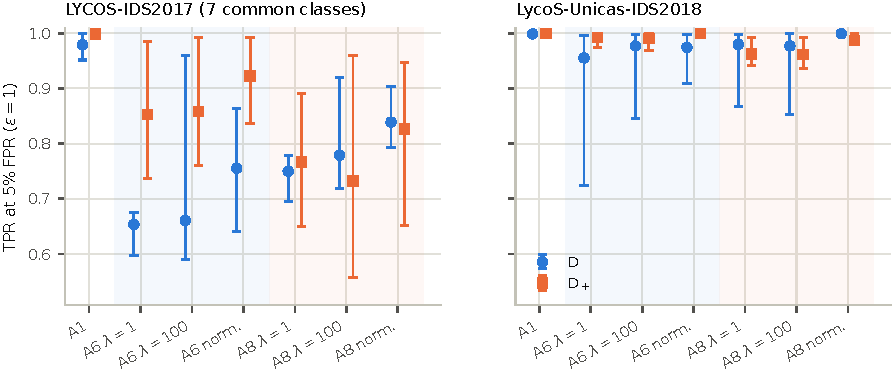
\includegraphics[width=\textwidth]{f_detection_tpr}
  \caption{TPR at \paramFPR{} FPR of D and D$_+$ per attack at $\epsilon = \paramEpsHead$, all source rows (V0); D$_+$
    against the stand-in attacker A8 (error bars: seed range).}
  \label{f_detection_tpr}
\end{figure*}

\begin{figure}[!tbp]
  \centering
  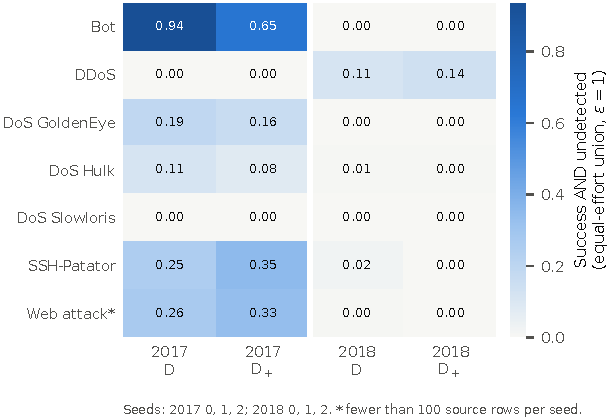
\includegraphics[width=\columnwidth]{f_per_class_heatmap}
  \caption{Per-class share of successful and undetected source rows under the equal-effort union at
    $\epsilon = \paramEpsHead$, all source rows (V0); D$_+$ against the stand-in attacker A8.}
  \label{f_per_class_heatmap}
\end{figure}

% Generated by paper_v3/gen/make_tables_v3.py on 2026-10-30. Do not edit.
% Source: results/stage9/a8x/summary_union.csv
% Source: results/stage9/adaptive/summary_union.csv
\begin{table}[t]
\centering
\footnotesize
\setlength{\tabcolsep}{4pt}
\caption{Against the stand-in attacker A8: equal-effort union with D$_+$ facing A1 + A8 $\times 3$ ($\epsilon = 1$), and the controls compared with D$_+$ under A8.}
\label{t_union_a8}
\textit{D$_+$ minus D, D$_+$ against A8}\par\smallskip
\sbox0{%
\begin{tabular}{llcccc}
\toprule
Dataset & Rows & Undet. D & Undet. D$_+$ & D$_+$ minus D [95\% CI] & Seeds 0 / 1 / 2 \\
\midrule
2017 & V0 & $0.246$ & $0.221$ & $-0.025$ {\scriptsize [$-0.039$, $-0.012$]} & $+0.063\,/\,-0.050\,/\,-0.089$ \\
2017 & V1 & $0.266$ & $0.229$ & $-0.037$ {\scriptsize [$-0.051$, $-0.023$]} & $+0.031\,/\,-0.058\,/\,-0.084$ \\
2017 & V2 & $0.293$ & $0.244$ & $-0.049$ {\scriptsize [$-0.064$, $-0.032$]} & $-0.004\,/\,-0.071\,/\,-0.071$ \\
\midrule
2018 & V0 & $0.023$ & $0.022$ & $-0.001$ {\scriptsize [$-0.008$, $+0.006$]} & $-0.050\,/\,+0.029\,/\,+0.018$ \\
2018 & V1 & $0.023$ & $0.022$ & $-0.001$ {\scriptsize [$-0.008$, $+0.007$]} & $-0.050\,/\,+0.029\,/\,+0.018$ \\
2018 & V2 & $0.029$ & $0.028$ & $0.000$ {\scriptsize [$-0.011$, $+0.009$]} & $-0.067\,/\,+0.040\,/\,+0.025$ \\
\bottomrule
\end{tabular}}%
\ifdim\wd0>\textwidth\resizebox{\textwidth}{!}{\usebox0}\else\usebox0\fi
\par\medskip
\textit{Control minus D$_+$, D$_+$ against A8 (V1)}\par\smallskip
\sbox0{%
\begin{tabular}{lllcccc}
\toprule
Dataset & Control & Attacker & Undet. control & Undet. D$_+$ & Minus D$_+$ [95\% CI] & Seeds 0 / 1 / 2 \\
\midrule
2017 & c0 & exact & $0.266$ & $0.229$ & $+0.037$ {\scriptsize [$+0.024$, $+0.052$]} & $-0.036\,/\,+0.060\,/\,+0.088$ \\
2017 & c1 & exact & $0.280$ & $0.229$ & $+0.051$ {\scriptsize [$+0.038$, $+0.066$]} & $-0.020\,/\,+0.057\,/\,+0.117$ \\
2017 & c2 & exact & $0.273$ & $0.229$ & $+0.045$ {\scriptsize [$+0.030$, $+0.060$]} & $-0.107\,/\,+0.139\,/\,+0.102$ \\
2017 & a1 & stand-in & $0.344$ & $0.229$ & $+0.115$ {\scriptsize [$+0.100$, $+0.130$]} & $+0.175\,/\,-0.054\,/\,+0.225$ \\
2017 & a2 & stand-in & $0.278$ & $0.229$ & $+0.050$ {\scriptsize [$+0.035$, $+0.065$]} & $-0.062\,/\,+0.026\,/\,+0.185$ \\
\midrule
2018 & c0 & exact & $0.015$ & $0.022$ & $-0.007$ {\scriptsize [$-0.014$, $-0.001$]} & $+0.041\,/\,-0.029\,/\,-0.034$ \\
2018 & c1 & exact & $0.019$ & $0.022$ & $-0.003$ {\scriptsize [$-0.009$, $+0.004$]} & $+0.044\,/\,-0.019\,/\,-0.034$ \\
2018 & c2 & exact & $0.055$ & $0.022$ & $+0.033$ {\scriptsize [$+0.024$, $+0.042$]} & $+0.001\,/\,+0.132\,/\,-0.034$ \\
2018 & a1 & stand-in & $0.006$ & $0.022$ & $-0.016$ {\scriptsize [$-0.021$, $-0.010$]} & $+0.010\,/\,-0.023\,/\,-0.034$ \\
2018 & a2 & stand-in & $0.021$ & $0.022$ & $-0.001$ {\scriptsize [$-0.007$, $+0.006$]} & $+0.040\,/\,-0.009\,/\,-0.032$ \\
\bottomrule
\end{tabular}}%
\ifdim\wd0>\textwidth\resizebox{\textwidth}{!}{\usebox0}\else\usebox0\fi
\par\smallskip\parbox{\linewidth}{\scriptsize D faces A1 + A6 $\times 3$. Paired bootstrap over source rows within seed (1,000 draws). These comparisons use the stand-in attacker A8 for D$_+$; against the exact-objective attacker A8x the sign of D$_+$ minus D reversed (Table~\ref{t_union_adaptive}), so the control minus D$_+$ values here are not the comparison at the stronger attacker.}
\end{table}

% Generated by paper_v3/gen/make_tables_v3.py on 2026-10-30. Do not edit.
% Source: results/stage9/a8x/summary_union.csv
% Source: results/stage9/a6x/summary_union.csv
\begin{table}[t]
\centering
\footnotesize
\setlength{\tabcolsep}{4pt}
\caption{D$_+$ minus D under A8x per attack setting, the unequal-effort sensitivity unions and the A6x union (V1, $\epsilon = 1$).}
\label{t_a8x_setting}
\sbox0{%
\begin{tabular}{llcc}
\toprule
Dataset & Union & D$_+$ minus D [95\% CI] & Seeds 0 / 1 / 2 \\
\midrule
2017 & A8x $\lambda{=}1$ vs A6 $\lambda{=}1$ & $+0.074$ {\scriptsize [$+0.059$, $+0.090$]} & $+0.152\,/\,-0.051\,/\,+0.121$ \\
2017 & A8x $\lambda{=}100$ vs A6 $\lambda{=}100$ & $+0.115$ {\scriptsize [$+0.099$, $+0.131$]} & $+0.204\,/\,+0.013\,/\,+0.128$ \\
2017 & A8x norm. vs A6 norm. & $+0.071$ {\scriptsize [$+0.054$, $+0.087$]} & $+0.169\,/\,-0.047\,/\,+0.090$ \\
2017 & Unequal effort: D$_+$ faces A1 + A8 $\times 3$ + A8x $\times 3$ & $+0.088$ {\scriptsize [$+0.074$, $+0.102$]} & $+0.137\,/\,-0.029\,/\,+0.155$ \\
2017 & A6x headline: D faces A1 + A6x $\times 3$ & $+0.075$ {\scriptsize [$+0.061$, $+0.090$]} & $+0.114\,/\,-0.037\,/\,+0.149$ \\
2017 & Unequal effort: D faces A1 + A6 $\times 3$ + A6x $\times 3$ & $+0.075$ {\scriptsize [$+0.061$, $+0.090$]} & $+0.114\,/\,-0.037\,/\,+0.149$ \\
\midrule
2018 & A8x $\lambda{=}1$ vs A6 $\lambda{=}1$ & $+0.007$ {\scriptsize [$+0.000$, $+0.014$]} & $-0.035\,/\,+0.016\,/\,+0.041$ \\
2018 & A8x $\lambda{=}100$ vs A6 $\lambda{=}100$ & $+0.012$ {\scriptsize [$+0.006$, $+0.018$]} & $-0.014\,/\,+0.010\,/\,+0.040$ \\
2018 & A8x norm. vs A6 norm. & $+0.003$ {\scriptsize [$-0.003$, $+0.009$]} & $-0.025\,/\,+0.026\,/\,+0.009$ \\
2018 & Unequal effort: D$_+$ faces A1 + A8 $\times 3$ + A8x $\times 3$ & $+0.016$ {\scriptsize [$+0.007$, $+0.024$]} & $-0.049\,/\,+0.053\,/\,+0.044$ \\
2018 & A6x headline: D faces A1 + A6x $\times 3$ & $+0.009$ {\scriptsize [$+0.001$, $+0.017$]} & $-0.050\,/\,+0.040\,/\,+0.039$ \\
2018 & Unequal effort: D faces A1 + A6 $\times 3$ + A6x $\times 3$ & $+0.009$ {\scriptsize [$+0.001$, $+0.018$]} & $-0.050\,/\,+0.040\,/\,+0.039$ \\
\bottomrule
\end{tabular}}%
\ifdim\wd0>\textwidth\resizebox{\textwidth}{!}{\usebox0}\else\usebox0\fi
\par\smallskip\parbox{\linewidth}{\scriptsize Per setting: D faces A1 and one A6 setting, D$_+$ faces A1 and the same A8x setting. Unequal effort: one side has twice as many candidates (marked); not a headline comparison. A6x: the A6 attack on D with the selection key of A8x (Section~\ref{sec:a6x}); separate bootstrap draws, so its interval can differ from the headline in the last digit.}
\end{table}

% Generated by paper_v3/gen/make_tables_v3.py on 2026-10-30. Do not edit.
% Source: results/stage9/a8x/summary_tpr.csv
\begin{table}[t]
\centering
\footnotesize
\setlength{\tabcolsep}{3pt}
\caption{Paired TPR and AUROC differences D$_+$ minus D on the rows of A8x and A8 ($\epsilon = 1$).}
\label{t_a8x_tpr}
\sbox0{%
\begin{tabular}{llcccccc}
\toprule
 &  & \multicolumn{2}{c}{V1} & \multicolumn{3}{c}{TPR difference [95\% CI]} & AUROC diff. \\
Dataset & Attack & Success & Undet. D$_+$ & V0 & V1 & V2 & V1 \\
\midrule
2017 & A8x $\lambda{=}1$ & $0.519$ & $0.282$ & {\begin{tabular}[t]{@{}c@{}}$-0.146$\\{\scriptsize [$-0.166$, $-0.125$]}\end{tabular}} & {\begin{tabular}[t]{@{}c@{}}$-0.175$\\{\scriptsize [$-0.203$, $-0.148$]}\end{tabular}} & {\begin{tabular}[t]{@{}c@{}}$-0.194$\\{\scriptsize [$-0.226$, $-0.164$]}\end{tabular}} & {\begin{tabular}[t]{@{}c@{}}$-0.037$\\{\scriptsize [$-0.044$, $-0.031$]}\end{tabular}} \\
2017 & A8x $\lambda{=}100$ & $0.438$ & $0.242$ & {\begin{tabular}[t]{@{}c@{}}$-0.152$\\{\scriptsize [$-0.177$, $-0.129$]}\end{tabular}} & {\begin{tabular}[t]{@{}c@{}}$-0.182$\\{\scriptsize [$-0.210$, $-0.154$]}\end{tabular}} & {\begin{tabular}[t]{@{}c@{}}$-0.213$\\{\scriptsize [$-0.246$, $-0.178$]}\end{tabular}} & {\begin{tabular}[t]{@{}c@{}}$-0.048$\\{\scriptsize [$-0.057$, $-0.039$]}\end{tabular}} \\
2017 & A8x norm. & $0.621$ & $0.252$ & {\begin{tabular}[t]{@{}c@{}}$-0.118$\\{\scriptsize [$-0.142$, $-0.095$]}\end{tabular}} & {\begin{tabular}[t]{@{}c@{}}$-0.124$\\{\scriptsize [$-0.150$, $-0.097$]}\end{tabular}} & {\begin{tabular}[t]{@{}c@{}}$-0.128$\\{\scriptsize [$-0.155$, $-0.099$]}\end{tabular}} & {\begin{tabular}[t]{@{}c@{}}$-0.051$\\{\scriptsize [$-0.058$, $-0.043$]}\end{tabular}} \\
2017 & A8 $\lambda{=}1$ & $0.524$ & $0.141$ & {\begin{tabular}[t]{@{}c@{}}$+0.016$\\{\scriptsize [$-0.005$, $+0.037$]}\end{tabular}} & {\begin{tabular}[t]{@{}c@{}}$+0.040$\\{\scriptsize [$+0.016$, $+0.067$]}\end{tabular}} & {\begin{tabular}[t]{@{}c@{}}$+0.072$\\{\scriptsize [$+0.042$, $+0.100$]}\end{tabular}} & {\begin{tabular}[t]{@{}c@{}}$+0.009$\\{\scriptsize [$+0.005$, $+0.014$]}\end{tabular}} \\
2017 & A8 $\lambda{=}100$ & $0.427$ & $0.125$ & {\begin{tabular}[t]{@{}c@{}}$-0.047$\\{\scriptsize [$-0.073$, $-0.022$]}\end{tabular}} & {\begin{tabular}[t]{@{}c@{}}$-0.017$\\{\scriptsize [$-0.046$, $+0.016$]}\end{tabular}} & {\begin{tabular}[t]{@{}c@{}}$+0.028$\\{\scriptsize [$-0.007$, $+0.063$]}\end{tabular}} & {\begin{tabular}[t]{@{}c@{}}$+0.006$\\{\scriptsize [$+0.002$, $+0.011$]}\end{tabular}} \\
2017 & A8 norm. & $0.620$ & $0.112$ & {\begin{tabular}[t]{@{}c@{}}$-0.012$\\{\scriptsize [$-0.031$, $+0.006$]}\end{tabular}} & {\begin{tabular}[t]{@{}c@{}}$+0.013$\\{\scriptsize [$-0.010$, $+0.036$]}\end{tabular}} & {\begin{tabular}[t]{@{}c@{}}$+0.049$\\{\scriptsize [$+0.023$, $+0.077$]}\end{tabular}} & {\begin{tabular}[t]{@{}c@{}}$+0.006$\\{\scriptsize [$+0.003$, $+0.010$]}\end{tabular}} \\
\midrule
2018 & A8x $\lambda{=}1$ & $0.336$ & $0.021$ & {\begin{tabular}[t]{@{}c@{}}$-0.037$\\{\scriptsize [$-0.055$, $-0.018$]}\end{tabular}} & {\begin{tabular}[t]{@{}c@{}}$-0.037$\\{\scriptsize [$-0.055$, $-0.019$]}\end{tabular}} & {\begin{tabular}[t]{@{}c@{}}$-0.052$\\{\scriptsize [$-0.079$, $-0.027$]}\end{tabular}} & {\begin{tabular}[t]{@{}c@{}}$0.000$\\{\scriptsize [$-0.005$, $+0.006$]}\end{tabular}} \\
2018 & A8x $\lambda{=}100$ & $0.317$ & $0.019$ & {\begin{tabular}[t]{@{}c@{}}$-0.032$\\{\scriptsize [$-0.050$, $-0.013$]}\end{tabular}} & {\begin{tabular}[t]{@{}c@{}}$-0.032$\\{\scriptsize [$-0.050$, $-0.015$]}\end{tabular}} & {\begin{tabular}[t]{@{}c@{}}$-0.042$\\{\scriptsize [$-0.066$, $-0.016$]}\end{tabular}} & {\begin{tabular}[t]{@{}c@{}}$-0.002$\\{\scriptsize [$-0.006$, $+0.003$]}\end{tabular}} \\
2018 & A8x norm. & $0.515$ & $0.016$ & {\begin{tabular}[t]{@{}c@{}}$-0.009$\\{\scriptsize [$-0.022$, $+0.002$]}\end{tabular}} & {\begin{tabular}[t]{@{}c@{}}$-0.009$\\{\scriptsize [$-0.021$, $+0.003$]}\end{tabular}} & {\begin{tabular}[t]{@{}c@{}}$-0.010$\\{\scriptsize [$-0.024$, $+0.004$]}\end{tabular}} & {\begin{tabular}[t]{@{}c@{}}$+0.009$\\{\scriptsize [$+0.004$, $+0.015$]}\end{tabular}} \\
2018 & A8 $\lambda{=}1$ & $0.335$ & $0.013$ & {\begin{tabular}[t]{@{}c@{}}$-0.017$\\{\scriptsize [$-0.031$, $-0.002$]}\end{tabular}} & {\begin{tabular}[t]{@{}c@{}}$-0.017$\\{\scriptsize [$-0.034$, $-0.003$]}\end{tabular}} & {\begin{tabular}[t]{@{}c@{}}$-0.026$\\{\scriptsize [$-0.047$, $-0.004$]}\end{tabular}} & {\begin{tabular}[t]{@{}c@{}}$0.000$\\{\scriptsize [$-0.003$, $+0.004$]}\end{tabular}} \\
2018 & A8 $\lambda{=}100$ & $0.324$ & $0.013$ & {\begin{tabular}[t]{@{}c@{}}$-0.016$\\{\scriptsize [$-0.032$, $-0.001$]}\end{tabular}} & {\begin{tabular}[t]{@{}c@{}}$-0.016$\\{\scriptsize [$-0.031$, $-0.001$]}\end{tabular}} & {\begin{tabular}[t]{@{}c@{}}$-0.022$\\{\scriptsize [$-0.042$, $+0.000$]}\end{tabular}} & {\begin{tabular}[t]{@{}c@{}}$+0.002$\\{\scriptsize [$-0.002$, $+0.007$]}\end{tabular}} \\
2018 & A8 norm. & $0.504$ & $0.006$ & {\begin{tabular}[t]{@{}c@{}}$-0.012$\\{\scriptsize [$-0.018$, $-0.007$]}\end{tabular}} & {\begin{tabular}[t]{@{}c@{}}$-0.012$\\{\scriptsize [$-0.019$, $-0.007$]}\end{tabular}} & {\begin{tabular}[t]{@{}c@{}}$-0.015$\\{\scriptsize [$-0.022$, $-0.009$]}\end{tabular}} & {\begin{tabular}[t]{@{}c@{}}$-0.001$\\{\scriptsize [$-0.002$, $-0.000$]}\end{tabular}} \\
\bottomrule
\end{tabular}}%
\ifdim\wd0>\textwidth\resizebox{\textwidth}{!}{\usebox0}\else\usebox0\fi
\par\smallskip\parbox{\linewidth}{\scriptsize TPR on the flipped rows at each detector's 5\% FPR threshold; AUROC against the benign test negatives; paired bootstrap, 1,000 draws. Both attacks were aimed at D$_+$, so negative values are expected by construction and are not evidence on their own. A8 intervals here come from the same pipeline as A8x and can differ in the last digit from Table~\ref{t_attacks}.}
\end{table}

% Generated by paper_v3/gen/make_tables_v3.py on 2026-10-30. Do not edit.
% Source: results/stage8/stage8c_standin_quality_2017.csv
% Source: results/stage7/stage7e/standin_quality.csv
% Source: results/stage9/adaptive/{2017,2018}/standin_quality.csv
\begin{table}[t]
\centering
\footnotesize
\setlength{\tabcolsep}{4pt}
\caption{Quality of the differentiable stand-ins ($R^2$ against the true score, mean over seeds): A8 for D$_+$ and the Stage B attackers of a1 and a2.}
\label{t_standin}
\sbox0{%
\begin{tabular}{lcccccc}
\toprule
 & \multicolumn{2}{c}{A8 (D$_+$)} & \multicolumn{2}{c}{a1} & \multicolumn{2}{c}{a2} \\
Consistency score & 2017 & 2018 & 2017 & 2018 & 2017 & 2018 \\
\midrule
rollout gxi spearman & $0.964$ & $0.948$ & $0.972$ & $0.958$ & $0.974$ & $0.959$ \\
rollout gxi jacc10 & $0.828$ & $0.840$ & $0.841$ & $0.859$ & $0.850$ & $0.866$ \\
rollout gxi cos & $1.000$ & $1.000$ & $1.000$ & $1.000$ & $1.000$ & $1.000$ \\
rollout ig20 spearman & $0.948$ & $0.928$ & $0.961$ & $0.945$ & $0.966$ & $0.950$ \\
rollout ig20 jacc10 & $0.820$ & $0.797$ & $0.845$ & $0.797$ & $0.835$ & $0.804$ \\
rollout ig20 cos & $0.983$ & $0.854$ & $0.990$ & $0.824$ & $0.987$ & $0.857$ \\
attnmean gxi spearman & $0.961$ & $0.948$ & $0.967$ & $0.952$ & $0.973$ & $0.950$ \\
attnmean gxi jacc10 & $0.807$ & $0.844$ & $0.834$ & $0.845$ & $0.855$ & $0.845$ \\
attnmean gxi cos & $1.000$ & $1.000$ & $1.000$ & $1.000$ & $1.000$ & $1.000$ \\
attnmean ig20 spearman & $0.954$ & $0.913$ & $0.963$ & $0.930$ & $0.967$ & $0.933$ \\
attnmean ig20 jacc10 & $0.809$ & $0.743$ & $0.833$ & $0.779$ & $0.850$ & $0.786$ \\
attnmean ig20 cos & $0.984$ & $0.870$ & $0.993$ & $0.857$ & $0.989$ & $0.891$ \\
\midrule
Median / min over features and seeds & $0.960$ / $0.756$ & $0.912$ / $0.652$ & $0.972$ / $0.800$ & $0.909$ / $0.726$ & $0.973$ / $0.803$ & $0.925$ / $0.736$ \\
\bottomrule
\end{tabular}}%
\ifdim\wd0>\textwidth\resizebox{\textwidth}{!}{\usebox0}\else\usebox0\fi
\par\smallskip\parbox{\linewidth}{\scriptsize Validation rows of each seed. a1 and a2: the 12 consistency columns of the control (x0 to x11, in the order of D$_+$); their four D features are exact. The last row covers the 12 consistency scores only, so it can differ from the $R^2$ in Table~\ref{t_union_adaptive}, which also covers the four exact D features. c0, c1 and c2 are attacked with exact gradients.}
\end{table}

% Generated by paper_v3/gen/make_tables_v3.py on 2026-10-30. Do not edit.
% Source: paper_v3/generated/numbers.tex (macros axRuns to sbInvalid; each macro names its result file)
\begin{table}[t]
\centering
\footnotesize
\setlength{\tabcolsep}{4pt}
\caption{Run records of the adaptive attacks added in this version: rows, validity, time, memory and sanity checks.}
\label{t_runs}
\sbox0{%
\begin{tabular}{lll}
\toprule
Quantity & 2017 & 2018 \\
\midrule
\multicolumn{3}{l}{\textit{A8x against D$_+$}} \\
Runs / rows / invalid rows & 18 / 18{,}261 / 0 &  \\
Minutes per run (attack and scoring) & 28~to~41 & 27~to~28 \\
Highest shared GPU memory / torch reserved (GB) & \ensuremath{0.076} / \ensuremath{4.45} &  \\
Sanity (a) and (b), other (c) checks: max abs. difference & \ensuremath{1.9 \times 10^{-6}} & \ensuremath{1.9 \times 10^{-6}} \\
Sanity (c) Mahalanobis, max rel. difference (tol. $10^{-3}$) & \ensuremath{2.4 \times 10^{-4}} & \ensuremath{6.2 \times 10^{-5}} \\
Sanity (c) D$_+$ decision, max abs. difference (tol. $10^{-3}$) & \ensuremath{2.1 \times 10^{-4}} & \ensuremath{2.1 \times 10^{-4}} \\
Run 1 (tol. $10^{-5}$, failed): Mahalanobis abs. / decision & \ensuremath{2.4 \times 10^{-3}} / \ensuremath{2.1 \times 10^{-4}} & not run \\
Flipped rows; undetected in loop without / with margin; evaluated & 5{,}355; 2{,}290 / 2{,}288; 2{,}290 & 3{,}453; 166 / 166; 166 \\
Max $|$in-loop $-$ evaluated D$_+$ score$|$, flipped rows & \ensuremath{3.5 \times 10^{-4}} & \ensuremath{3.2 \times 10^{-4}} \\
\midrule
\multicolumn{3}{l}{\textit{A6x against D}} \\
Runs / rows / invalid rows & 18 / 18{,}261 / 0 &  \\
Seconds per run & 58~to~83 & 43~to~64 \\
Highest shared GPU memory / torch reserved (GB) & \ensuremath{0.076} / \ensuremath{4.15} &  \\
Sanity (s1), selection off, chunk 500: max abs. difference & \ensuremath{0} & \ensuremath{0} \\
Run 1 (chunk 50, failed (s1)): max abs. difference; rows & \ensuremath{1.4 \times 10^{4}}; 3 & not run \\
Rows with a different kept iterate / all rows & 11{,}589 / 18{,}261 &  \\
Rows whose flipped / undetected status changed & 0 / 0 &  \\
\midrule
\multicolumn{3}{l}{\textit{Stage B, controls under their own adaptive attackers}} \\
Runs / rows / invalid rows & 90 / 91{,}305 / 0 &  \\
\bottomrule
\end{tabular}}%
\ifdim\wd0>\textwidth\resizebox{\textwidth}{!}{\usebox0}\else\usebox0\fi
\par\smallskip\parbox{\linewidth}{\scriptsize Where only the 2017 column is filled, the value covers both datasets. Sanity checks compare the quantities computed inside the attack with the saved values on the sanity rows of seed 0 (results/stage9/a8x and a6x, log\_sanity.txt). Run 1 of A8x failed at tolerance $10^{-5}$ from single-precision noise; the tolerance and the 1e-3 selection margin were amended before any pilot or attack. Run 1 of A6x failed at chunk 50 from the batch shape of the forward passes; the chunk was set to that of A6 before any A6x attack (Section~\ref{sec:a6x}).}
\end{table}

